\documentclass[twoside]{article}
\let\nofiles\relax 
\usepackage{amsfonts,amssymb,amsbsy,textcomp,marvosym,picins,amsmath,caption,threeparttable,amsthm,subfigure}
\usepackage{eurosym,mathrsfs,fancyhdr,CJK,multicol,graphics,indentfirst,color,bm,upgreek,booktabs,graphicx}
\usepackage{multirow,enumitem}
\usepackage{longtable}
\usepackage{lscape}
\usepackage[hyperref=true,backend=biber,sorting=none,backref=true]{biblatex}
\addbibresource{graph.bib}
%\usepackage[noend]{algorithm}
%\usepackage[noend]{algorithmic}
%\usepackage[lined,algonl,boxed]{algorithm2e}
\looseness=-1
%------------Page layout and margin and Headrule-------------
\headsep=5mm \headheight=4mm \topmargin=0cm \oddsidemargin=-0.5cm
\evensidemargin=-0.5cm \marginparwidth=0pt \marginparsep= 0pt
\marginparpush=0pt \textheight=23.1cm \textwidth=17.5cm \footskip=8mm
\columnsep=7mm \setlength{\doublerulesep}{0.1pt}
\renewcommand{\thefootnote}{\fnsymbol{footnote}}
\footnotesep=3.5mm\arraycolsep=2pt
\font\tenrm=cmr10
%===========================================================
\def\footnoterule{\kern 1mm \hrule width 10cm \kern 2mm}
\def\rmd{{\rm d}} \def\rmi{{\rm i}} \def\rme{{\rm e}}
\def\sj#1{$^{[#1]}$}\def\lt{\left}\def\rt{\right}
\renewcommand{\captionfont}{\footnotesize}
\renewcommand\tablename{\bf \footnotesize Table}
\renewcommand\figurename{\footnotesize Fig.\!\!}
\captionsetup{labelsep=period}%
\captionsetup[longtable]{labelsep=period}%
\allowdisplaybreaks
\sloppy
\renewcommand{\headrulewidth}{0pt}
\catcode`@=11
\def\title#1{\vspace{3mm}\begin{flushleft}\vglue-.1cm\Large\bf\boldmath\protect\baselineskip=18pt plus.2pt minus.1pt #1
\end{flushleft}\vspace{1mm} }
\def\author#1{\begin{flushleft}\normalsize #1\end{flushleft}\vspace*{-4pt} \vspace{3mm}}
\def\address#1#2{\begin{flushleft}\vglue-.35cm${}^{#1}$\small\it #2\vglue-.35cm\end{flushleft}\vspace{-2mm}\par}
\def\jz#1#2{{$^{\footnotesize\textcircled{\tiny #1}}$\footnotetext{$^{\footnotesize\textcircled{\tiny #1}}$#2}}}
\def\jzd#1#2{$^{\footnotesize\textcircled{\tiny{#1}}}$\footnotetext{$^{\footnotesize\textcircled{\tiny{#1}}}$#2}}
\catcode`@=11
\def\section{\@startsection{section}{1}{\z@}%
 %{-3.5ex \@plus -1ex \@minus -.2ex}%
 {-3ex \@plus -.3ex \@minus -.2ex}%
 {2.2ex \@plus.2ex}%
{\normalfont\normalsize\protect\baselineskip=14.5pt plus.2pt minus.2pt\bfseries}}
\def\subsection{\@startsection{subsection}{2}{\z@}%
 %{-3.25ex\@plus -1ex \@minus -.2ex}%
 {-3ex\@plus -.2ex \@minus -.2ex}%
 {2ex \@plus.2ex}%
{\normalfont\normalsize\protect\baselineskip=12.5pt plus.2pt minus.2pt\bfseries}}
\def\subsubsection{\@startsection{subsubsection}{3}{\z@}%
 %{-3.25ex\@plus -1ex \@minus -.2ex}%
 {-2.2ex\@plus -.21ex \@minus -.2ex}%
 {1.4ex \@plus.2ex}
{\normalfont\normalsize\protect\baselineskip=12pt plus.2pt minus.2pt\sl}}
\def\proofname{{\indent \it Proof.}}
%===========================================================���ϲ���

\pagestyle{fancy}
\fancyhf{}% ����ҳüҳ��
\fancyhead[LO]{\small\sl First Author {\it et al.}: Shortened Title Within 45 Characters}%
\fancyhead[RO]{\small\thepage}
\fancyhead[LE]{\small\thepage}
\fancyhead[RE]{\small\sl J. Comput. Sci. \& Technol., January 2018,
Vol., No.}
\setcounter{page}{1}
\begin{document}
\begin{CJK*}{GBK}{song}
\thispagestyle{empty}
\vspace*{-13mm}
\noindent {\small First Author, Second Author, Third
Author {\it et al.} Journal of computer science and technology: Instruction for authors.
JOURNAL OF COMPUTER SCIENCE AND TECHNOLOGY \ 33(1): \thepage--\pageref{last-page}
\ January 2018. DOI 10.1007/s11390-015-0000-0}
%===========================================================
\vspace*{2mm}

\title{Graph Processing Accelerators: A Survey}

\author{First Author[\textcolor{blue}{First-Name Surname}]$^{1,2,*}$, Second Author$^{1}$, and Third Author$^{2}$}

\address{1}{Institute of Computing Technology, Chinese Academy of Sciences, Beijing 100190, China}
\address{2}{[\textcolor{blue}{Affiliation, City Postcode, Country}]}

\vspace{2mm}

\noindent E-mail: ***@*********; ***@********* [\textcolor{blue}{Please list the emails of all the authors in order}]\\[-1mm]

\noindent Received July 15, 2018 [\textcolor{blue}{Month Day, Year}]; revised October 14, 2018 [\textcolor{blue}{Month Day, Year}].\\[1mm]

\footnotetext{{}\\[-4mm]\indent\quad Regular Paper\\[.5mm]
%\indent\quad Special Section of CAD/Graphcis 2017\\[.5mm]
%\indent\quad  A preliminary version of the paper was published in SMP 2014.\\[.5mm]
\indent\quad by the National Natural Science Foundation of China under Grant Nos.~******** and ********, the National High Technology Research and Development 863 Program of China under Grant No.~********, the National Basic Research 973 Program of China under Grant No.~********, and the Natural Science Foundation of Shandong Province of China under Grant No.~*******. \\[.5mm]
\indent\quad$^*$Corresponding Author
%\\[1.2mm]\indent\quad $^{\footnotesize\textcircled{\tiny1}}$
\\[.5mm]\indent\quad \copyright 2018 Springer Science\,+\,Business Media, LLC \& Science Press, China}

\noindent {\small\bf Abstract} \quad  Graph processing accelerators can significantly improve the performance and energy efficiency of graph analytics which are important for big data analysis. These accelerators often utilize various kinds of emerging architectures and frameworks. However, it is hard to extract a clear thread for the designs because of the diverse characteristics and complexity. Moreover, there are no corresponding review literatures offering a systematical view of design for graph processing accelerator. This paper aims to point out the considerations for graph processing accelerators designs. In this paper, the necessity and the importance of graph processing accelerators are firstly introduced in details. Next, the procedure of graph processing design is presented as three phases: preprocessing of graph datasets, graph parallel computation, runtime scheduling. In addition, the evaluation results of different kinds of graph processing accelerators are discussed from different aspects. Finally, challenges and opportunities of graph processing accelerators are presented for the future. 

c{\small \textcolor{blue}{Please provide an abstract of 100 to 250 words. The abstract should clearly state the nature and significance of the paper. It must not include undefined abbreviations, mathematical expressions or bibliographic references.}}

\vspace*{3mm}

\noindent{\small\bf Keywords} \quad {\small graph processing, accelerator, architecture, parallel computation

keyword [\textcolor{blue}{Keywords should closely reflect the topic and should optically
characterize the paper. Please use about 3$\sim $5 keywords or phrases in
alphabetical order separated by commas.}]}

\vspace*{4mm}

\end{CJK*}
\baselineskip=13.2pt plus.2pt minus.2pt
\parskip=0pt plus.2pt minus0.2pt
%%%%%%%%%%%%%%%%%%%%%%%%%%% Main Text Begin %%%%%%%%%%%%%%%%%%%%%%%%%%%%%%%%%
\begin{multicols}{2}

%intruduction
\section{Introduction}
Recent years have seen the explode of information amount in every area. Graphs are expressive to represent the relationship among various kind of data in social networks, roads map and genomics area. Graph processing thus become a hot topic in both academic research and industry applications. With the growing development of Internet of Things and cloud computing, the size and complexity of graphs are increasing. There's a need to pursue efficient technologies to deal with the challenges of graph processing.

To make graph processing more efficient under such enormous amount of data size, there has already been a lot of graph processing frameworks. From distributed computing systems \cite{Malewicz2010pregel, low2012graphlab} to those based on single high-end server \cite{Shun2013ligra} or commercial PC \cite{Kyrola2012graphchi, Roy2013x-stream}. And there are systems focusing on performance of special graph algorithms \cite{liu2015enterprise}. Basically, these systems pay efforts to software optimizations for programmability, high performance and scalability under traditional architectures. To accelerate graph processing workloads, GPU is adopted for its high degree of parallelism. Works such as Cusha \cite{khorasani2014cusha}, GunRock \cite{Wang2016gunrock}, Frog \cite{shi2018frog}, MapGraph \cite{Fu2014mapgraph}, Enterprise \cite{liu2015enterprise} have achieved high performance. 

There has already been a lot of mature good experience on software graph processing. However, the performance can be bounded by inefficiencies of current architectures. The real-world graphs typically follow a power-law rule, and has intuitive irregular access patterns with strong dependency between nodes. So it always comes with a high memory access overhead and low efficiency of using the traditional memory hierarchy in traditional general purpose processors such as the caches. And it's hard to explore the memory and instruction level parallelism of graph processing. When applying emerging memory devices, it's also difficult to fully utilize the bandwidth under traditional CPUs. GPUs also have difficulties to solve problems such as control and memory divergence, load imbalance and huge amounts of global memory accesses for its architectures designed for regular workloads. Energy efficiency is another key issue for graph processing in big data era as the amount of graph workloads keep on increasing. However, CPUs and GPUs are known for relatively high energy cost. It's rather difficult to make more progress on performance or energy efficiency under current architectures.

Customized graph processing accelerators have been proved to be a promising solution to achieve both high performance and energy efficiency \cite{ham2016graphicionado,Dai2017foregraph,ahn2015tesseract} because of the dedicated processing units and efficient memory hierarchies. 

Hennessy and Patterson have identified the trend and opportunities for computer architectures. Huge benefits can be gained from domanin-specific architectures (DSAs) \cite{DSA}. The free and open architectures and open-source implementations make it easier for innovations on hardware design \cite{DDFCP,RISCV, ERI}. The agile chip development will also shorten the developing time and cost for accelerator prototypes \cite{AGILE, ADH}. To maintain high performance and energy efficiency. Many industries have already deployed customized accelerators such as FPGAs and specific AISCs to accelerate their analytic workloads. Microsoft \cite{microsoftazure}, Amazon \cite{aws-ec2} have been using FPGAs to accelerate their data-centers. It is a trend to explore the domain-specific accelerators for graph processing.

\vspace{2mm}

\begin{center}
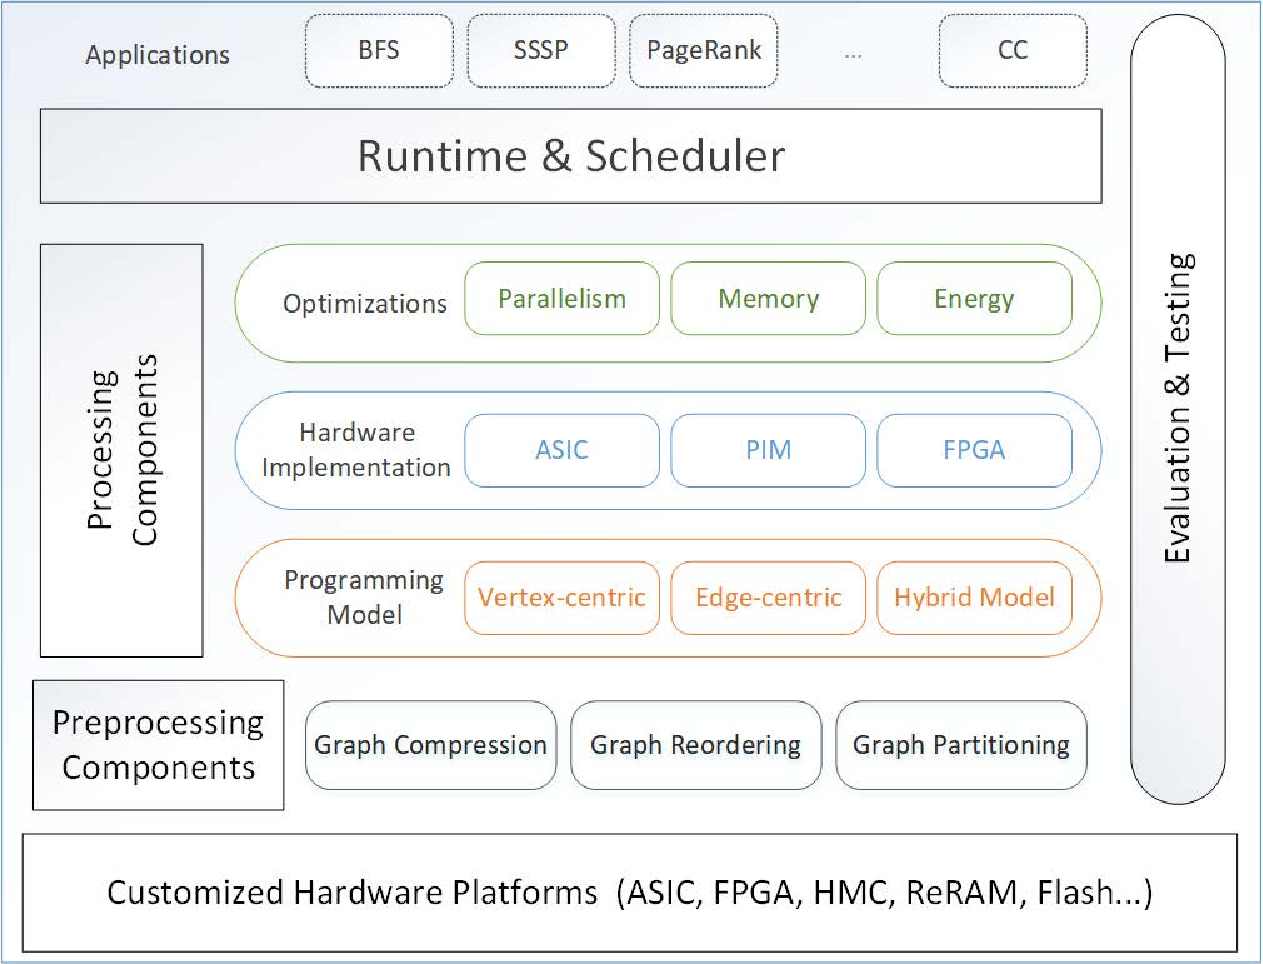
\includegraphics[width = 8cm]{pictures/graphacc.pdf}\\
\vspace{2mm}
\parbox[c]{8.3cm}{\footnotesize{Fig.1.~}  Building blocks of graph accelerator. }%\vspace*{.2mm}
\end{center}

\vspace{1mm}

In this article we survey a large number of typical works on graph processing accelerators. It aims to explore the key issues and general procedure to build a graph accelerator. Several issues need to be considered according to the normal progress of graph processing from preprocessing phase to runtime and scheduler as shown in Figure 1.

\begin{itemize}
\item \emph{Preprocessing.}
Preprocessing is an important issue that operate on the graph data to make it fit into the space on accelerators and suitable for processing models before processing. Generally, the storage resources are limited on accelerators and graphs need to be partitioned, different kinds of architectures may also require specific representations of graph to run correctly.

\item \emph{Processing components.}
Processing components act as the main parts of accelerator design. Generally, programming models are chosen to define the basic pattern for execution of vertices and edges which are mapped to the hardware. Different kinds of hardware architectures can be selected to build the graph accelerator such as ASICs, PIM and FPGAs. These architectures have their own concerns during the design. Besides, optimizations can be adopted to further improve the performance an energy efficiency.

\item \emph{Runtime Scheduling.}
The runtime systems and scheduler in the graph accelerators are important components to guarantee the correctness and efficiency of execution. 
\end{itemize}


We also analyze the trend of graph processing accelerators and propose some challenges and opportunities in the future. The challenges comes from many aspects. For example, the programmability is an important issue for users to express their graph applications. Existing accelerators are lack of efficient support for this, heavy labour are need for hardware level modifications. There are other challenges such as the support for dynamic graph processing and completeness of graph primitives. The opportunities for graph processing accelerators should be seen as well. Widespread graph applications and applied situations push for energy-efficient graph processing accelerators. Emerging memory devices such as HMC \cite{hmc}, HBM \cite{hbm}, ReRAM \cite{reram} along with new processing devices provide us with many opportunities to explore new schemes for graph processing.

The rest of the paper is organized as follows: Section 2 includes a introduction to basic components of graph processing, and typical progress on CPUs and GPUs. Section 3 presents some considerations in preprocessing phase. Several important components considered in processing phase are explained in section 4. Section 5 describe the runtime and scheduler part of graph accelerators. Some emerging graph accelerators are compared in section 6.  Challenges and opportunities of graph processing accelerators are promoted in section 7. Finally, we conclude our work in section 8.


\section{Preliminaries}
%Graph data and graph algorithms are two key components of graph processing. 
In this section, we first give a brief introduction to some preliminaries for helping understand graph processing. Afterwards, a number of unique characteristics of graph processing have been summarized, followed by on limitations of graph processing on commodity processors, further motivating our survey on graph accelerators in this work.

\subsection{Graph Representation}
Graph is a data structure consisting of nodes that are further associated with edges. A typical graph can be defined as $G = (V, E)$ where $V$ represents the vertices and $E$ indicates the edges. For a directed graph, its edge can be represented as $e=(v_i, v_j)$, indicating that there's an edge pointing from $v_i$ to $v_j$. In particular, vertex and edge can be also attributed with a single or a set of data.

Natural graphs such as relationships in Facebook usually have three common features. The first one is the sparse graph structure which means the average degree of vertices is at a low level. The sparsity of graphs can result in poor locality. The second one is the power-law distribution which means only a few vertices are connected with most of the edges. This can cause severe workload imbalance issue and result in many conflicts when proess the high degree vertex. The third one is the small-world structure that two random vertices are connected to each other from only a few hops. The small-world feature will make it difficult for efficient graph partitioning.

\subsection{Graph Algorithms}
We present several common graph algorithms with different complexities in computation, communication as well as memory requirements.

{\bf Traversal-centric Algorithms}\quad This kind of algorithms usually require traversing the graphs from specific vertices in a certain way. Usually there is a frontier array maintains the active vertices. The memory accesses to computations ratio is high. In the meanwhile, it requires a lot of random accesses which leads to a big pressure of memory bandwidth. 

{\em Breadth-First Search} (BFS) is a basic graph traversal algorithm and used as the kernel by Graph500 benchmark. The neighbors are iteratively accessed from the root vertex until all the vertices of graph are visited. Heavy random accesses to vertices and edges exist in each iteration.

{\em Single Source Shortest Path} (SSSP) is another graph traversal algorithm that computes the shortest paths from a source vertex to other vertices in the graph. Different from BFS, it has less waste in checking edges and each vertex may be activated more than once. It also needs more memory space than BFS.

{\em Betweenness Centrality} (BC) algorithm is widely used to measure the importance of a vertex in a graph. The betweenness centrality value of a vertex is calculated by the ratio of shortest paths between any other two vertices that contain the vertex. BC algorithm requires computing the shortest paths between all pairs of vertices which puts more pressure on memory bandwidth.

{\bf Compute-centric Algorithms}\quad Different from traversal-centric algorithms, compute-centric algorithms require more computations in a iterative way. All the vertices are often activated in each iteration. This kind of algorithms usually present better locality than traversal-centric algorithms. However, float-point computations are often needed.

{\em PageRank} algorithm is one of the most popular algorithm that calculates the scores of and websites, which is proposed by Google. It maintains a PageRank value for each vertex, usually represent as a float point number. All the vertices are activated in each iteration, which put more pressure on memory bandwidth and float point computing ability.

{\em Connected Components} (CC) algorithm is widely used in image regions analysis and clustering applications. Each vertex maintains a label that if vertices are in the same connected region, their labels are set to the same. The algorithm iteratively updates the labels of all the vertices until convergence.

{\em Triangle Counting} (TC) algorithm is used to measure the number of triangle cliques in the graphs which are common in social networks. Each vertex maintains a list of its neighbors and iteratively check if there are shared neighbors between each connected pair of vertices. The number of triangles is calculated by the overlaps.

\subsection{Unique Features of Graph Processing}
%{\color{blue}
%list the features of graph processing which are challenging for accelerator %design.
%}
As demonstrated before, the real-world graphs typically have the "small-world" feature and "power-law" distribution. In other way, the graph algorithms differs in computational and memory access requirements. The complexity of graph data and the algorithms together make graph processing a challenging task which typically have below features.

\emph{\bf Intensive Data Access:} Graph applications usually result in huge amounts of data accesses requests. Besides, graph processing has a high data access to computation ratio where most of the operations in graph processing are related to data accesses which consumes most of the time during the procedure.

\emph{\bf Irregular Computation:} Due to the power-law distribution, computation workloads for different vertices may vary in a large scale. This will result in severe workload imbalance issue and communication problems.

\emph{\bf Poor Locality:} Data accesses in graph processing are usually in a random pattern because of each vertex may connected to any other random vertex through the whole graph. The issue can result in heavy overhead in memory accesses.

\emph{\bf High Data Dependency:} The data dependency is caused by the nature of connections of vertices in graph. Heavy dependencies make it difficult to explore the parallelism in graph processing and may cause frequent data conflicts which drag down the performance.

\subsection{Related Work: Graph Processing on Modern Commodity Processors}

Many graph processing systems have been explored on modern commodity processors as CPUs and GPUs.

{\bf Graph Processing on CPUs}\quad
There have been lots of works aim to build an efficient environment for graph applications on CPUs. Basically, they can be divided into two categories. The first kind is the distributed systems \cite{Malewicz2010pregel, Gonzalez2012powergraph,giraph,Gonzalez2014graphx, teixeira2015arabesque, chen2015powerlyra, Zhu2016gemini} which leverage the clusters to support huge amounts of data. But developing under the distributed environment usually suffers a lot from communication cost, synchronization overhead, fault tolerance and load imbalance issues \cite{khayyat2013mizan,randles2010comparative,zhao2014lightgraph,wang2014replication}. Emerging servers can hold most of the graph data in its large memory. So there are works exploit the potential of single machine to process large graphs \cite{Shun2013ligra, nguyen2013galois, sundaram2015graphmat,Zhang2015numa-aware}. There are also many disk-based graph processing systems proposed \cite{ Kyrola2012graphchi, Roy2013x-stream, han2013turbograph, yuan2014pathgraph, zhu2015gridgraph, chi2016nxgraph} which can avoid above challenges of distributed systems. Recently, MIC architecture (Many Integrated Core Architecture) based processors are also explored to improve the performance of graph processing \cite{Maass2017mosaic}.


{\bf Graph Processing on GPUs}\quad
GPU is adopted to pursue higher performance of graph processing for its intuitive higher parallelism and high bandwidth that outperform CPUs. A number of graph processing systems \cite{Wang2016gunrock,khorasani2014cusha,zhong2014medusa,seo2015gstream} have been proposed to run high-performance graph processing with GPUs. GPUs are first used to accelerate specific graph algorithms. Enterprise \cite{liu2015enterprise} is developed
based on the BFS algorithm and GPU characteristics. There are also works on fast connected components \cite{soman2010fast}, betweenness centrality implementations \cite{mclaughlin2014scalableBC,pande2011computingBC,sariyuce2013betweenness} and single-source shortest path algorithms \cite{davidson2014work}. Domain-specific graph processing frameworks have been researched to provide higher efficiency for generic graph processing development on GPUs \cite{Hong2012green-marl}. To support larger scale of graphs, hybrid CPU-GPU systems \cite{gharaibeh2013totem, zhang2015ggraph}, multi-GPUs systems \cite{liu2016ibfs, ben2017groute} and out-of-memory systems \cite{sengupta2015graphreduce, kim2016gts} have been researched.

{\bf Remark}\quad
Existing works on CPUs and GPUs can provide abundant experience for designs of graph accelerators. For effectively expressing graph applications in a generic framework, various kinds of graph processing models have been proposed. For supporting large scale graphs, strategies such as partitioning methods, out-of-memory processing and hybrid architectures schemes have been explored. 

These experience can help to build the graph accelerators. Generally, customized graph accelerators have relatively fixed circuits designs thus efficient programming models are needed to support various kinds of applications. The storage capacities on graph accelerators are limited so the partitioning methods from those single machine can be referred to handle large graphs. Basically, to improve the performance and energy efficiency, it's important to combine these experience with dedicated hardware designs. We will illustrate the main considerations when build a graph accelerator in the successive sections.


\section{\textcolor{red}{Graph pre-processing}}
%{\color{blue}
%preprocessing mainly include three parts, the %compression and reordering of graph %representations for different need. partitioning %because of the limited storage space on %accelerators. preprocessing is for graph data.
%}
%Because of the limited capacity of on-chip memory on hardware accelerators, most of the real-world graphs cannot be directly placed on chip for the graph processing. Preprocessing serves as an important component, which usually involves compressing, reorganizing and partitioning the graph data according to the storage capacity and processing models. This makes it possible to process the large-scale graphs on limited on-chip memory. This section reviews three kinds of useful approaches on the preprocessing of graph datasets for different demands.
Graph data is usually huge and critical to the graph processing. In order to adapt the data structure to the target graph accelerators, people usually perform pre-processing on the original graph data for the sake of higher performance. In this section, we will investigate the major graph preprocessing techniques used in graph accelerator design. 

\subsection{Graph Data Layouts}
%{\color{blue}
%There are different kind of graph representations, and sorting is needed for graph store.
%}
The graph preprocessing usually starts from the baseline graph layouts, so we will introduce 
baseline graph layouts first. There are generally 
two widely adopted baseline graph layouts i.e. the edge array and compressed 
adjacency list. For edge array based graph, each element of the array contains 
a pair of integers i.e. source vertex index and destination vertex index. 
It is convenient to be read from files to memory for stream processing 
and remains widely used in many graph processing systems especailly 
the edge-centric systems. A similar layout is {\bf Coordinate List} (COO) 
and it has been adopted in a few graph accelerators 
\cite{song2018graphr,zhou2016highthroughput,Dai2017foregraph}. 
The major difference is that it has the edge property stored 
along with each edge i.e. vertex pair.  

Compressed adjacency list graph orignates 
from the adjaceny matrix. It typically uses three arrays to store the 
graphs i.e. the vertex property array of the graph, the edge array with 
only the edges' outgoing/incoming vertex indeices and the edge array starting indices 
of each vertex in the graph. When outgoing edges are used in the edge array, 
it is named as compressed sparse row (CSR). When incoming edges are used 
in the edge array, the layout is called compressed 
sparse column (CSC). The compressed adjacency list graph is relative compact and 
beneficial to many graph accelerators \cite{ozdal2016energy,Zhang2017fpgahmcbfs}. 
In addition, the edges are stored contiguously and can be accessed in an efficient 
sequential pattern.

%An intuitive method to store a graph is to use an {\em adjacency matrix} where each row represents a source vertex and the column represents the destination vertex. Each value in the matrix represents the edge value. For the graph datesets that are generally sparse, this method is prone to store many useless zero value which wastes considerable storage spaces. 
%While this representation is direct and easy to access and modify, it cost extremely large storage space which is impractical to place the graphs on graph accelerators. 
%For example, for a graph with $n$ vertices and $m$ edges, it cost $O(n^2)$ storage space. Due to the sparsity of graph data structure, it may contain many redundant value existing in the matrix. 
%For better storing more valid values on the limited on-chip memory, people seeks the solutions with compressed storage formats.
%Compressed representations such as compressed sparse row (CSR) and coordinate list (COO) are needed to represent the graphs in a more efficient way.
On top of the two baseline graph data layouts, there are many other graph layouts that 
require more processing efforts. In this survey, we 
take them as graph data layout pre-processing. For instance, the authors in proposed to associate the 
destination vertex property with the edge information \cite{Oguntebi2016graphops} such that the vertex 
property accesses show much better locality. Another layout optimization proposed in \cite{attia2014cygraph} 
is to modify the row pointer array representation of that in a typical CSR format. It combines the 
vertex status (1 bit for BFS only) and the vertex's neighboring information in the same array 
in a compact manner. This method improves the memory access efficiency significantly. 
Different from the above methods, some of the researchers optimize the layout through more efficient 
encoding. For example, the graph may not be equal to the number of all vertices thus the indices can be compressed to a relatively smaller scale by remove the blank vertices \cite{dai2018graphh}. The index can be compressed by grouping them and using a coarsen id which cost less bits to represent \cite{Dai2017foregraph,ham2016graphicionado}. The edge information can be further compressed by encoding methods based on the frequency of vertices in the edge list \cite{Zhang2018degreebfsfpga}.

{\bf Remark}
Despite the benefits on storage space. The compression can bring other drawbacks and need some optimizations for better use. The CSR format have the problem of randomly accessing to destination vertices. The COO format can also cause random accesses to both the source and destination vertices. Besides, it usually caused redundant edge accesses. This can be solved by dedicated partitioning methods \cite{Dai2017foregraph}.

Dedicated compression of graph data can help to utilize the limited storage space on accelerators more efficiently. They also improve the locality of graphs which is important for graph accelerator to reduce the memory access overhead. Because of the less required data size, bandwidth can be saved and provide higher performance.

\subsection{Graph Reordering}
Reordering is usually used to avoid the data conflicts and guarantee the correctness of execution \cite{zhou2016highthroughput,han2017reram}. It can also improve the locality of graph data to improve performance. It's usually done by first reassign IDs to vertices and edges according to the new order while maintain the original structure of graphs, then the graph data is stored according to the new order.

{\bf Index-aware Reordering}\quad Edges can be sorted according to the index order of either the source vertex or the destination vertex. Sorting the edges in an ascending manner of their source vertex IDs \cite{dai2018graphh} can improve the data reuse of source vertex. Sorting the edges in an ascending manner of the destination vertex IDs can optimize the updates of destination vertices and reduce the writing overhead \cite{zhou2016highthroughput}. The source and destination ID can be considered together to furtherly optimize the processing \cite{Dai2016fpgp,Dai2017foregraph,ham2016graphicionado}. 

{\bf Degree-aware Reordering}\quad Vertices and edges can be sorted according to the degree information. Usually, high degree vertices are more likely to be accessed by other vertices, it can improve the locality and compression rate by reordering the vertices in the order of descending degrees \cite{Zhang2018degreebfsfpga}. The edge array in CSR format can be sorted according to the degree of destination vertices to improve locality for the same reason \cite{Khoram2018fpgaco-optimizinghmc}. The degree-aware reordering can help balance the workloads as well \cite{Zhou2018fastcf}.

{\bf Other Reordering Methods}\quad The reordering methods can be sophisticated to help optimize the processing phase. For example, the order of edges are organized in an interleaving style to improve the parallelism of memory access in ForeGraph \cite{Dai2017foregraph}. These reordering methods are usually related to other execution designs. 

{\bf Remark} It's note that not all of the accelerators need reordering methods. However, by utilize this method flexibly, performance can be significantly improved.

One drawback of reordering method is the time consumption when sort the graphs. Once the size of graphs become large, the preprocessing time will be unignorable. Some accelerators design special units to process the sorting during the process phase to achieve better performance \cite{song2016novelspmv,yao2018pact,JUN2018GRAFBOOST}, in this way the latency can be covered by interleaving with other operations.

\subsection{Graph Partitioning}
%{\color{blue}
%Partitioning is used to make graphs fit into the %accelerators' chips
%}
Graph partitioning is an effective way to divide a whole large graph into many small subgraphs that can be fit into accelerator memory. 
%The partitioning is adopted by many graph accelerators where only subgraphs can be fit into the storage space of chips due to the limited hardware resources. 
Graph partitioning can be also used to exploit the potential parallelism between different processing units. 
%To partition a graph, both of the vertices and edges need to be considered. Vertices are partitioned into individual intervals with edges associated in a partition based on different kind of partition strategies. Generally, 
Existing graph partitioning strategies basically can fall into four categories below.

\tabcolsep 12pt
%\cmidrule(l){2-4}%
\renewcommand\arraystretch{1.3}
\begin{center}
{\footnotesize{\bf Table 1.} Partitioning Schemes of Graph Accelerators}\\
\vspace{2mm}
\footnotesize{
\begin{tabular*}{\linewidth}{lp{4cm}p{4cm}}\hline\hline\hline
Partitioning Schemes & Graph Accelerators
\\\hline
Source-Oriented & {\cite{9,11,15,22,29,34,40}} \\
Destination-Oriented &  {\cite{1,4,12,13,26}} \\
Grid like & {\cite{10,30,39}} \\
Heuristic & {\cite{2,5,6,7,25,37,38}}
\\\hline\hline\hline
\end{tabular*}%\vspace*{.2mm}
\\\vspace{1mm}\parbox{8.3cm}{}
}
\end{center}

\vspace{1mm}

\textbf{Source-oriented Partition}\quad 
The source-oriented partition methods typically work in the following way. The vertices are first divided into multiple disjoint subsets. Then the edges are distributed to according subsets having the source vertices \cite{zhou2016highthroughput,yao2018pact}. This kind of partition associates the out edges of each vertex in the same partition, thus the locality of source vertices can be explored when processing the edges. Considering of the graph representations mentioned before, it can be easily realized by divide the CSR or COO into different sets. 

For example, an interval-shard like partition method is used by several works \cite{zhou2016highthroughput,zhou2017cpufpga}. In \cite{zhou2016highthroughput} the vertices are evenly partitioned according to the storage space on FPGAs. The edge list are partitioned as mentioned before and sorted by the destination vertices. During the execution, the vertex subset of each partition is transferred to the on-chip block RAMs (BRAMs) while the edges are streamed from DRAM to the chip and processed using the source vertices and the edge values. 


{\bf Destination-oriented Partition}\quad 
Similar to the source-oriented partition methods, the destination-oriented partition \cite{Dai2016fpgp,ham2016graphicionado} first dived the vertices into several intervals and the in-edges of the vertices in each subset are associated to the same partition. The advantage of this kind of partition is that the destination vertices can be reused and keep a good locality.

For example, Graphicionado \cite{ham2016graphicionado} use the hash method to evenly partition the vertices, the partitions are processed and updated sequentially while the destination vertices are stored on the scratchpad to fully utilize the locality. GraphP \cite{zhang2018graphp} uses this kind of partition significantly reduce the communications among different accelerators because there are less messages need to be sent from the source vertex.

{\bf Grid-like Partition}\quad
Grid like partition first evenly partition the vertices into different subsets \cite{Dai2017foregraph,song2018graphr}, the adjacency matrix are then partitioned into a grid divided by these subsets. Any two vertex subsets and according edge block in the grid form a partition. This kind of partition can provide a finer grained partitions than simply source-oriented or destination-oriented ones and can keep both of the locality of source vertices and the destination vertices. 

Fore example, ForeGraph \cite{Dai2017foregraph} design caches for the vertex subsets on FPGA boards and stream the edges of each block to the processing units which significantly optimize the memory accesses. The locality of vertices are fully explored during the execution. GraphR \cite{song2018graphr} used grid like partition to utilize the computing power of ReRAM and achieved high performance. 

{\bf Heuristic Partition}\quad
Different from previous three kinds of partitioning methods which explicitly partition the graph into subgraphs. Heuristic partition methods usually adopt some heuristic algorithms or tools to partition the graph for different goals such as better locality and load balance. 

For example, Hash algorithms are commonly used to evenly partitions the vertices and the edges \cite{ozdal2016energy}. Clustering algorithms are used to partition the graph into subgraphs with good locality \cite{Khoram2018fpgaco-optimizinghmc}. Multi level partitioning is adopted in FASTCF \cite{Zhou2018fastcf} to furtherly improve the effect of partitioning.

{\bf Remark}
There are some considerations for better use of partitioning methods. It's important to balance the workloads in different partitions. The vertex subsets can be partitioned according to the degrees to evenly distributed the edges. Sophiscated partitioning methods also have a trade-off between the efficiency and time consumption. These partitioning methods can also be integrated in hardware to improve the performance.

The preprocessing phase provide a basis for the following processing phase. The efficiency of preprocessing can significantly influence the performance. We will present main considerations of processing phase in next section.

\section{Graph Parallel Processing}
After graph preprocessing, the key of next step is how to handle these preprocessed graph data with massive parallellism. Considering intertwined data dependencies of graphs, this often requires three layers of technical innovations with matched parallel programming models, dedicated hardware acceleration as well as sophisticated software co-optimizations.% for better performance, lower memory overhead and energy consumption.

\subsection{Programming Models}
Graph structure has complex data dependencies between vertices. Programming model is an effective way that can decouple these associated dependencies as much as possible by exploring the common computation pattern surrounding vertices and/or edges. Existing programming models for graph processing can be basically divided into two subcategories: vertex-centric model and the edge-centric model. A few graph accelerators also have made a hybrid attempt for embracing the best of both worlds in vertex- and edge-centric programming models.

\tabcolsep 12pt
%\cmidrule(l){2-4}%
\renewcommand\arraystretch{1.3}
\begin{center}
{\footnotesize{\bf Table 2.} Programming Models of Graph Accelerators}\\
\vspace{2mm}
\footnotesize{
\begin{tabular*}{\linewidth}{lp{4cm}p{4cm}}\hline\hline\hline
Programming Model & Graph Accelerators
\\\hline
Vertex-Centric & {\cite{1,2,4,5,6,7,8,9,10,12,15,16,17,18,19,20,21,22,25,26,27,32,33,36,37,40,41}} \\
Edge-Centric &  {\cite{10,13,23,24,28,29,30,38,39}} \\
Hybrid & {\cite{34}} 
\\\hline\hline\hline
\end{tabular*}%\vspace*{.2mm}
\\\vspace{1mm}\parbox{8.3cm}{}
}
\end{center}

\vspace{1mm}

{\bf Vertex-centric Model} Graph algorithms using this model handle the graphs by following "Think like a vertex" philosophy  \cite{Malewicz2010pregel,bu2014pregelix}. It handles a vertex program per vertex, including the computational operations and data transmission between their neighbors via edges. Since the each vertex can be processed independently, parallelism can be guaranteed by simultaneously scheduling those vertices without data dependencies.

Vertex-centric model has been widely used to drive many graph accelerators \cite{nurvitadhi2014graphgen,ozdal2016energy,ham2016graphicionado,Dai2016fpgp} because of its expressive potentials to easily represent various kind of graph algorithms, and high parallelism in the grain of vertex. However, in the vertex-centric model there can be random accesses to edges, resulting in potentially heavy memory access overhead. %Optimizations are usually needed as illustrate in later sections. 


{\bf Edge-centric Model}\quad
X-Stream \cite{Roy2013x-stream} is the first to use edge-centric model to handle graph edges. Unlike the vertex-centric model, this model thinks like an edge. It handles the graph datesets per edge. During the graph processing, an edge program is applied to each edge by collecting the information of its source vertices, updating its value, and sending this value to its destination vertices. It is clear that this model removes the random accesses to edges via sequential streaming of each edge to the chips. 

Edge-centric model is usually used by existing graph accelerators for improving the utilization of their limited memory bandwidth \cite{zhou2016highthroughput,Dai2017foregraph, Zhou2018fastcf}. However, the point is that edge-centric model is lack of flexible scheduling potentials in contrast to the vertex-centric model. Almost all of edges have be processed multiple times to complete the whole process of graphs. In addition, this model may also lead to much random accesses to vertices. Thus, additional optimizations are often co-operatively needed, e.g., fined grained partitioning and tailored update strategies \cite{Dai2017foregraph,song2018graphr}.

{\bf Hybrid Programming Model}\quad
Alternative is to use a hybrid method by switching between vertex- and edge-centric programming models for the purpose of taking advantages of both models. This model is adopted in \cite{zhou2017cpufpga}, targeting graph algorithms in which only a subset of vertices are processed during each iteration.

The switching time between these two models is decided by the active vertex ratio in each iteration which cause a trade-off between random memory accesses in vertex-centric model and redundant edge checks in edge-centric model. When the active vertex ratio in a iteration is low, then vertex-centric paradigm is adopted because of smaller random memory accesses and less redundant edge checks. When the active vertex ratio is high, the edge-centric one is used. To apply the hybrid model, graphs are partitioned into vertex intervals and edge shards. These partitions can be applied with different programming models and switch between two models independently according to the switching scheme. Besides, an array of edge offsets in the COO is needed to record the first outgoing edge of each vertex.



{\bf Implementation of Programming Interfaces}
The programming models just define the pattern of execution of graph algorithms in vertex or edge programs, it is important to find ways to implement these programs for graph accelerators. No matter the graph program is based on either vertex or edge, their execution semantics can be usually implemented in three ways as follows according to the number of synchronization phases for each program:

\underline{\em One-phase Execution Model}: In one phase execution model, the vertex programs work as a single function and executed in a bulk synchronous parallel (BSP) mode \cite{Malewicz2010pregel, betkaoui2012fpgabfs}. The computations are executed in supersteps, there is a barrier between two supersteps to synchronize the vertex programs. Each vertex iteratively using the information of its neighbors and edges to update itself and send updates to the outgoing edges. This model is used because it is easy for vertex programs to run in parallel and implemented in accelerators. However, it may result in workload imbalance issue.

\underline{\em Two-phase Execution Model}: Two phase models are widely used in both vertex- and edge-centric models and it is adopted by most of the accelerators \cite{Roy2013x-stream,ham2016graphicionado}. In this model, the vertex program is broken down into two functions and synchronizations are needed for each function. Scatter-Gather execution model is a commonly used two-phase model. Scatter function calculate with source vertices and out-edges then propagate the new values along the edges. Gather function collects computation information from in-edges and update the destination vertices. The two-phase execution model can be used to decouple the computations and updating phases. In this way, the random memory accesses can be reduced compared to one-phase execution model.

\underline{\em Three-phase Execution Model}: Three phase execution models usually divide the vertex program into three functions, this kind of execution model can be executed in both synchronous and asynchronous way. Three-phase model usually means the GAS (Gather-Apply-Scatter) \cite{Gonzalez2012powergraph, ozdal2016energy}. Gather function accumulate the information from in-edges. Apply function do the computing and update operation. Then the Scatter function propagate the new values through out-edges. GAS model can decouple the data transfer and computations to achieve finer parallelism. This model simplifies the expression of vertex program. When implemented in graph accelerator, it cost less efforts for users to design their own programs.  



{\bf Summary}
Both the vertex- and edge-centric models can be used to represent various kinds of graph applications and thus suit for graph accelerators to handle different graph problems. The vertex-centric models are mostly used in these accelerators because it is more easier for users to describe the execution pattern of graph algorithms and easier to implement on graph accelerators. Besides, it can provide flexible scheduling potentials of vertices for graph accelerators. However, the random accesses to edges of this model will cause degradation of memory bandwidth utilization which become a bottleneck for graph accelerators that limit the performance. Edge-centric model is adopted because it remove the random accesses to edges which can significantly improve the performance by fully utilizing the bandwidth of graph accelerators. Besides, the edge-centric model suit more for some special computing devices such as the ReRAM \cite{Han2018reram} according to the storage pattern of edges. However, redundant edge checks are usually difficult to avoid because the edges are streamed from the memory to chips. Besides, it causes more random accesses to vertices. Basically, there is a trade-off existing in both models between the random access and sequential access. 

There are various kinds of programming models in existing software graph processing frameworks that can be referred to. Due to the complexity of hardware design, the programming models need to be simple, expressive and efficient. More efficient programming models can be explored for graph accelerators.


\subsection{Dedicated Hardware Acceleration}

Existing graph processing accelerators are basically built upon three types of hardware platforms: Field Programmable Gate Array (FPGA), Application-Specific Integrated Circuit (ASIC), and Processing-in-Memory (PIM). Different platforms have different considerations for the performance acceleration. We next analyze the features of different hardware platforms and review existing efforts of graph processing accelerators based on them.

\subsubsection{FPGA-based Graph Accelerators}
FPGA is an integrated circuit that enables designers to repeatedly configure digital logic in the fields after manufacturing, thus also called {\em field-programmable}. The configuration of FPGAs is generally specified via low-level hardware description languages, such as Verilog \cite{thomas2008verilog} and VHDL \cite{ashenden2010designervhdl}. FPGAs are mostly adopted in graph accelerators.

{\bf Internal Characteristics of FPGAs}\quad There are various kinds of programmable resources on FPGAs such as  programmable logic elements (LEs), static random access memory (SRAM or Flash) and block RAMs (BRAMs), however these resources are usually limited to a small amount.

FPGA can offer high parallelism using these resources, generally  processing on FPGA follows a pipeline MISD model where many functional circuits perform different operations on the same data in a pipeline stream. Multiple data can be processed at different stage at the same time. Different pipelines can be easily connected through hardware resources on FPGA boards to achieve higher parallelism. 

{\bf Existing Efforts on FPGAs}\quad 
To implement graph processing on a FPGA board, processing units and the memory subsystem should be designed. A graph algorithm is usually designed into a circuit kernel as basic processing unit according to the programming model which defines the execution pattern of a vertex or edge \cite{betkaoui2012ssspbrain, Zhou2018fastcf}. These kernels can be easily mapped into different algorithms due to the reconfigurable feature of FPGAs. As for the memory subsystem, existing work mainly focus on the efficient utilization of on-chip BRAMs and the off-chip memory bandwidth. BRAMs provide high bandwidth and low memory latency for randomly accessed vertices. By dedicated partitioning mechanisms, the locality of vertices on the BRAM is improved \cite{Dai2016fpgp, Dai2017foregraph, Zhang2018degreebfsfpga}. The utilization of off-chip bandwidth can be improved by adopting edge-centric programming model and increasing the pipelines for memory access \cite{zhou2016highthroughput}.

The flexible architectures of FPGAs can be utilized to scale the power of single FPGA board due to abundant interface resources on FPGAs. Multiple FPGAs can be combined into clusters to process large graphs with connected network to achieve high bandwidth \cite{Zhang2017fpgahmcbfs, attia2014cygraph}. FPGAs with integrated soft-cores are explored to improve the performance of graph processing \cite{kapre2015softcorefpga}. Heterogeneous architectures are also used to improve the performance of graph processing \cite{zhou2017cpufpga}. There are also a number of studies that aim to explore the out-of-memory execution on FPGAs for larger graphs \cite{Dai2016fpgp, Dai2017foregraph}. Recently, near data processing (NDP) are cooperatively used to enhance the power of FPGAs for graph processing \cite{Khoram2018fpgaco-optimizinghmc,Zhang2017fpgahmcbfs,JUN2018GRAFBOOST}.




% ASIC
\subsubsection{ASIC-based Graph Accelerators}
ASIC is an integrated circuit composed of electrical components, such as resistors, usually fabricated on a wafer composed of silicon or other semiconductor material that is customized for a particular use. ASICs are very compact, fast, and low power. Compared to FPGAs, their functions are hard-wired at the time of manufacture, it is not allowed to change the functionality of a small part of the circuit. 

{\bf ASIC Designs for Graph Analytics}\quad 
Due to the fixed circuit limitation, ASIC based graph accelerators usually utilize the expressive GAS model to form the circuits frameworks \cite{zhou2017tunao,ozdal2016energy}. Each phase is implemented as a hardware module and run in parallel with wires connecting different modules. In order to support various graph algorithms, a reconfigurable block can be integrated for users to define the update functions. 

As for the memory hierarchy, the ASIC based graph accelerators commonly adopt the scrathpad memory to replace traditional cache. The scrathpad memory acts as a content addressable cache and can be controlled manually. Graphicionado \cite{ham2016graphicionado} uses eDRAM as the scratchpad memory to store graph data that needs frequent random accesses, such as the destination vertices. Dedicated caches of different kinds of graph data are designed in \cite{ozdal2016energy} according to the access features. Since these memory resources can be tightly connected to the processing units in an efficient way, ASIC-based graph accelerators can achieve high throughput on chip. 

% Emerging device
\subsubsection{PIM-enabled Graph Accelerators}
Processing-in-Memory architecture is an emerging technology in which the processing units are tightly integrated into the memory and can benefit from the extremely high bandwidth and low memory access latency with energy saving. The PIM-enabled acceleration is often implemented by leveraging emerging memory devices, e.g., Hybrid Memory Cube (HMC) and REsistive Random Access Memory (ReRAM), both of which integrate the in-situ computation in the memory.

{\bf HMC-assisted Graph Processing}\quad The HMC has multiple DRAM dies stacked on top of a logic layer that can provide the ability of computation with high memory access parallelism and sufficient instructions for supporting graph processing. The DRAM dies are connected via through-silicon-via (TSV). Storage space in HMC is organized as vault. It is a vertically connected stack of multiple partitions from different DRAM layers. The logic layer is also distributed to different vaults. With multiple DRAM channels for each vault, HMC can provide significantly higher memory-level parallelism than traditional DRAM and the ability for processing in memory. HMC can also be easily scaled to consist of a cluster of HMC topology for better efficiency and energy.

The logic layer of each vault can work as a soft-core with sufficient instruction sets. For better supporting graph processing, instructions have to be re-constructed. Tesseract \cite{ahn2015tesseract} integrate common instructions of graph algorithms and achieve high performance through multiple HMCs. GraphPIM \cite{nai2017graphpim} deigns specialized atomic instructions in HMCs. Besides, graphs are processed in a distributed manner among HMCs and vaults. Strategies, such as vertex-cut partitioning, are used to reduce the communication cost \cite{zhang2018graphp, dai2018graphh}.

{\bf ReRAM-assisted Graph Processing} The resistive random access memory (ReRAM) is a kind of non-volatile RAM enabled the compute ability by changing the resistance across a dielectric solid-state material \cite{reram}. A ReRAM cell is with high density, low read latency and high energy efficiency \cite{reram2}. The ReRAM cells can be connected as a dense crossbar architecture to provide high parallelism and memory capacity. Generally, the graph can be represented as a matrix which can be easily mapped to ReRAM cells. Each cell stores an edge or a vertex of the graph, when input voltages are applied to certain rows of the cells array, the stored values of each row will multiply the relevant input value and then the stored values of each columns will be added together. These computations are common when graph algorithms are mapped to matrix operations. These features make it possible to realize efficient graph processing on ReRAM.

The potential of ReRAM for efficient computation and storage is still under-studied significantly. To our best knowledge, GraphR \cite{song2018graphr} is the first work to use ReRAM to speedup the graph processing. It transfers vertex program or edge program in graph processing to sparse matrix-vector multiplication (SpMV) format. {\bf introduce the principle of GraphR here}. However, the graph algorithms need to be manually justified for mapping the computing pattern of ReRAM. It is worth noting that there is also a tradeoff between the utilization and throughput due to the limited ReRAM size. Larger size of ReRAM is needed to achieve higher parallelism and throughput. However, due to the sparsity of graph data and constrained storage format, there may be only small number of edges in the ReRAM block thus the many ReRAM cells is underutilized. Tailored efforts are needed to balance the tradeoff.

{\bf Summary}
Considering reconfigurable feature, FPGA-based design can handle various kind of graph algorithms flexibly. FPGA can also provide sufficient interfaces to process large graphs for scale-out efficiency. Massive parallelism can be easily achieved when these resources are in good use. Unfortunately, the resources on FPGAs are limited to existing commodity FPGA boards provided by the producers. For example, the fixed type of memory devices and constrained circuits placement. The frequency is also relatively low to maintain correctness of execution. These may influence the performance in some extent.

ASIC design can provide more flexible and efficient hardware organizations without the limitation on types and amounts of hardware resources compared to FPGAs. Thus the ASICs can be designed in a more imaginative and efficient way. For example, dedicated and accurate resources placement can be achieved while the FPGAs usually have redundant and wasted resources on board. Besides, the ASIC can achieve a higher frequency than FPGAs thus high performance can be easily attained. However, once made, the ASIC chip is unable to be modified. It is usually difficult for ASICs to handle various graph problems. It is also difficult for ASICs to scale out.

PIM based accelerators can scale well with both of the bandwidth and memory capacity. This feature can benefit the graph processing when larger graphs are handled. The emerging memories adopted in PIM based accelerators usually have lower energy consumption than traditional DRAM which is important for energy efficient graph processing. To handle generic graph analytics, the HMC provides the compute ability by special instruction sets execute in the logic layer. ReRAM process the graphs in the SpMV format with corssbars. These supports usually need many manual efforts to realize. There are still lots of spaces for PIM based accelerators. For example, the bandwidth can be underutilized due to the communication overhead in HMCs. ReRAM can also be underutilized due to the sparsity of graphs. 

Different kinds of graph processing accelerators have their own features on hardware architectures and developing methods. They can all achieve high performance and energy efficient graph processing when designed deliberately. It is also promising to combine these accelerators together to achieve better behaviour. 

\subsection{Sophisticated Co-optimization}
Generally speaking, graph accelerators often need a series of specialized optimizations for fully exploiting their hardware potentials.
There also emerge a few co-optimization techniques at these aspects for higher parallelism, lower memory access overhead, and better energy-efficiency.

\subsubsection{Parallelism Extension}
The processing units in either ASIC- or FPGA-based graph processing accelerators are often organized in the form of {\em pipeline}. The instructions of graph algorithms are pipelined to offer high parallelism. PIM based graph accelerators integrate the processing units inside the memory. Their efficency can be scaled by simply enlarging the memory capacity. For better scalability, three optimization solutions below can be considered useful potentially.

{\bf Pipeline Replication}\quad An intuitive method to increase the throughput is to replicate multiple pipelines for the parallel processing on more vertices and edges. This simple method has been widely used in a wide spectrum of previous work~\cite{ham2016graphicionado,ozdal2016energy,zhou2017tunao,song2016novelspmv,betkaoui2011graphlet,zhou2016highthroughput,zhou2015fpgasssp}. Nevertheless, there still remain some potential problems that might prevent the scalable efficiency of multi-pipeline from expectation, which is significantly under-studied. For instance, 
considerable communication between pipelines may lead to the additional overhead via crossbars and controllers~\cite{ham2016graphicionado,ozdal2016energy}. In addition, there also exists workload balance issue that needs specialized data partitioning~\cite{Dai2017foregraph,ham2016graphicionado}.

{\bf Split Kernel} Alternative is to split a big, whole processing stream into many small kernels that can be then considered being executed in parallel. This is often done by decoupling the modules of data access and computation, and then making them executed in parallel. In this way the data access module is responsible for accessing graph data. The computation module uses the data to conduct user-defined computations. 
For example, by using gather-apply-scatter (GAS) model, \cite{ozdal2016energy,zhou2017tunao,attia2014cygraph} create specialized circuits for each phase. Each module thus enables to process large nubmer of vertices and edges concurrently. The SpMV based accelerator \cite{song2016novelspmv} also decouples the matrix access from the computation. This method aims at exploring the task-level parallelism but extra scheduling mechanism are needed to ensure the correctness.

{\bf Using Dataflow Paradigm}\quad Vertex dependencies of graph can stall the pipelines and decrease the instruction level parallelism. How to reduce the impact arising from data dependencies remains an open problem for increasing the number of instructions per cycle (IPC). 
One viable solution for sovling this problem is to leverage dataflow paradigm~\cite{jin2017dataflow,Oguntebi2016graphops}, which form a directed graph of the operations according to data dependency between two adjacent operations \cite{jin2017dataflow}. The output dependency and control dependency in graph processing can be thus significantly eliminated \cite{jin2017dataflow}. GraphOps \cite{Oguntebi2016graphops} uses dataflow model to form the data path of different processing blocks thus the overhead of control feedback is alleviated.

\subsubsection{Memory Access Optimization}
For graph processing, it is observed that memory accesses often dominate overall execution time. Designing efficient memory subsystem is crucial for the graph processing accelerator, particularly for memory access efficiency \cite{ham2016graphicionado, ozdal2016energy}. Below is most commonly used optimizations for enhancing the performance of memory access.

{\bf Enhancing Memory-level Parallelism} (MLP) This method can be represented as the number of outstanding memory requests supported at the same time. Higher memory level parallelism can reduce the total memory access time for data-intensive applications as graph processing. It usually needs the memory devices to support enough concurrent memory requests. There are two ways to enhance the MLP.

\textit{Multiple Banks} One method to increase the MLP is using multiple banks. DRAM is composed of many independent banks, utilizing the parallelism of these banks can significantly improve the memory level parallelism \cite{betkaoui2011graphlet,betkaoui2012fpgabfs,betkaoui2012ssspbrain}. The memory banks are connected to the processing units directly through point-to-point crossbars and can be accessed concurrently in these accelerators. Thus huge amounts of memory accesses can be satisfied.

\textit{Multiple I/O Ports} Another method is designing multiple I/O ports for a memory block \cite{nurvitadhi2014graphgen,zhou2016highthroughput,zhou2015fpgasssp}. By increasing the I/O ports, multiple memory requests can run concurrently. Usually the number of ports can be manually organized on scratchpad memory (SPM), high MLP can be attained when the number of ports are equal to the number of processing units \cite{ham2016graphicionado}. BRAMs on FPGAs can also be manually controlled to achieve this goal \cite{zhou2016highthroughput}. These BRAMs are usually combined together to form a memory block with multiple I/O ports.

{\bf Improving Bandwidth Utilization }\quad The memory bandwidth utilization here means the valid values ratio per transfer to and from the memory. Random accesses in graph processing usually caused low ratio of valid values and result in much wasted bandwidth. Improving the memory bandwidth utilization can reduce the total number of memory accesses thus reduce the execution time. There are mainly two effective methods to improve the bandwidht utilization.

\textit{Coalescing Method} Coalescing means combining multiple transfers of small items into fewer large ones, which reduces the pressure of memory bandwidth. This method is widely adopted in graph accelerators \cite{nurvitadhi2014graphgen,zhou2016highthroughput,zhou2015fpgasssp,zhou2015fpgapagerank,Zhang2017fpgahmcbfs}. For example, if the memory requests are adjacent in a vertex or edge list. Then these requests can be coalescing as one request for a block. Otherwise there may exist several random accesses that cause waste of bandwidth \cite{nurvitadhi2014graphgen}.

\textit{Streaming Edges} Streaming edges means that the edges are sequentially accessed from the memory to accelerator chips \cite{zhou2016highthroughput, Roy2013x-stream}, thus random accesses to edges can be reduced which may result in heavy memory access overhead. In a vertex-centric model, the edges of a vertex can be streamed to the chip \cite{ham2016graphicionado}. This method can fully utilize the bandwidth in the edge-centric model because the edges fetched are all processed, the edges may need to be reordered to run more efficiently \cite{Dai2017foregraph,zhou2016highthroughput}.

{\bf Reshaping Cache Architecture}\quad Poor locality of graph processing makes the current cache hierarchy lack of efficiency. High cache miss rate will increase the memory access latency and put more pressure on the bandwidth, which also cause the underutilization of computing resources. Reshaping the cache architectures means designing new cache hierarchy and mechanism according to the features of graph processing.

\textit{Scratchpad Memory} Scratchpad Memory (SPM) is used as an addressable cache that can be explicitly controlled. SPM is closed to the graph engines thus can provide high performance for data access \cite{Windh2015fpgacam,dai2018graphh}. Graphicionado \cite{ham2016graphicionado} use SPM to store the temporary vertex property array and edge offset to optimize the random data accesses. Similarly, \cite{ozdal2016energy} also designs different kind of caches for vertices, edges and other graph information according to their access behaviors. 

\textit{Locality-aware Buffer} Locality-aware buffer is specialized cache for for graph data with relatively good locality such as the high degree vertices. High degree vertices in a power-law graph have more potential to be accessed many times, these vertices can be cached to improve performance \cite{zhou2017tunao}. FPGP \cite{Dai2016fpgp} and ForeGraph \cite{Dai2017foregraph} improve the locality of vertices using grid-like partitioning methods and design special on-chip cache for these vertex subsets thus the subset can be accessed fast for reuse.

\textit{Execution-aware Prefetching} The execution-aware prefetching prefetch the graph data according to the execution requirements, thus avoid the inefficiency of fixed traditional cache prefetching mechanism.  For example, in vertex-centric model, the source vertex list and according edge list can be prefetched sequentially while the random accesses one need to be prefetched according to buffered messages \cite{ahn2015tesseract}. The key is to exploit the access patterns of different kinds of graph data during the execution and design appropriate prefeching mechanism to cover the memory latency.




\subsubsection{Energy-efficiency Optimization}
Energy-efficiency can be measured by Traversed Edges Per Second and per Watt (TEPS/W). Existing graph processing accelerators can provide significantly high performance by dedicated designed circuits with  inherently low energy consumption thus the energy-efficiency can be improved. However, most graph applications has high memory access to computation ratio. For example, the power breakdown results show that PageRank consumes over 60\% energy on memory \cite{guo2015pimenergy}. Optimizations on memory power can furtherly improve the energy efficiency in a large extend. There are two ways to optimize the memory power.

%The main energy cost reside in the memory for the data-intensive nature of graph processing. So, saving the power consumption of memory is vital to building an energy efficient graph accelerator. 

{\bf Leveraging Emerging Memory Technologies} A number of emerging memory technologies integrate the compute logic inside the memory, such as HMC~\cite{ahn2015tesseract, nai2017graphpim, zhang2018graphp,dai2018graphh} and ReRAM~\cite{song2018graphr,huang2018hyve} as described previously. This architectural reformation can conduct the in-situ computation along side the data, thus naturally avoiding the frequent data movement for energy saving. 
At this point, we thus can replace traditional DRAM by leveraging these emerging memory devices. %These accelerators adopt emerging memory devices which have natural low power consumption than traditional memory devices such as HMC  and ReRAM . HBM is also another good choice.

{\bf Power-gating Scheme} Power-gating is a widely used technology that power-off the idle logic circuits to save the energy. This scheme suits for memories that can be manually controlled \cite{zhou2016highthroughput, huang2018hyve}. For example, it can be applied to BRAMs on FPGAs that dominates the overall FPGA energy consumption in graph processing accelerators \cite{zhou2016highthroughput}. The BRAM is selectively activated and deactivated via the enable port \cite{fpgapower}. A BRAM module is only activated when the required data is stored in it. When the edges of a vertex are stored in the same BRAM module, the BRAM only need to be activated once to traverse these edges \cite{zhou2016highthroughput}. Similar strategy can be used for ReRAM \cite{huang2018hyve} to save the energy for edge accesses by controlling the activation of ReRAM banks.

\section{Runtime Scheduling}
{\color{blue}
}
Specially-designed hardware accelerator often requires tailored runtime scheduling to make the desired data in the appropriate place. Traditional runtime scheduling . Unlike the runtime scheduling based on traditional processors, the runtime scheduler on graph accelerator is generally implemented as hardware circuit that can control the data flow in the accelerators and the terminal of processing. 
%The runtime can be composed of various kinds of modules. The counters, memory controllers, crossbars and schedulers can all become part of the runtime which depend on the processing designs. 
Making such a specific runtime scheduling on graph accelerator needs to consider three properties at least.
\begin{itemize}[leftmargin=*]
\item {\em Correctness}. When edges and vertices are processed concurrently, conflicts occur because of the dependencies. Typically the data dependency occurs when a vertex wait for its neighbors' values or the same vertex is accessed by multiple processing units. By dedicatedly designed synchronous units SYU \cite{ozdal2016energy} using priority scheduling mechanism to guarantee the correctness and support an asynchronous execution model. Zhou \cite{zhou2015fpgasssp,zhou2016highthroughput} uses data forwarding method within the pipeline and a sorting module to reduce the influence of data dependency.

\item {\em Workload Balance}. the workloads between different processing units. This usually need static scheduling mechanism based on graph partition to distribute the workloads evenly. Graphicionado \cite{ham2016graphicionado} uses Hash method to distributed the workloads and schedules the vertices and edges by crossbars. 

\item {\em Execution Model}. Asynchronous execution are supported in \cite{ozdal2016energy} using priority scheduling mechanism. Scheduler is designed in \cite{zhou2017cpufpga} to switch between the push and pull style \cite{umuroglu2015hybridbfsfpga} or between the CPU and FPGA \cite{zhou2017cpufpga}.
\end{itemize}

For the sake of ensuring these properties, the following typical runtime scheduling strategies are proposed based on different granularity for different purposes. 
{\bf Vertex-oriented Scheduling}
This kind of scheduling is basically applied to vertices and usually exist in the vertex-centric model. The accelerators typically maintain an frontier array and a state array for the vertices. The frontier contains the active vertices which need to be executed. The scheduler get information based on vertices in the frontier and check the state array to decide the data path of different vertices. The vertices can be assigned a rank as the priority to make sure the correctness of parallel execution of different tasks. Vertex-oriented scheduling can provide fine-grained control of the execution of vertices and can be easily scheduled during runtime.

{\bf Edge-oriented Scheduling}
Edge-oriented scheduling mechanism is usually adopted in the edge-centric model. The edges are usually streamed from the DRAM to the accelerators. So the scheduling usually based on the order of the edges. When the edges are distributed to different streams to process, to reduce conflicts, the edges can be shuffled to offer better parallelism \cite{Dai2017foregraph}.

{\bf Subgraph-oriented Scheduling}
Subgraph-oriented scheduling is based on graph partitioning methods. During the processing, the subgraphs are scheduled between the accelerators and DRAM to complete the process. For interval-shard partitioning, the shards are processed one by one \cite{zhou2016highthroughput}. To provide finer granularity of scheduling and improve the locality of vertices, ForeGraph \cite{Dai2017foregraph} partitions the graph into grid, and schedule the blocks in the grid during the processing. These blocks can be divided into sub-blocks to distributed to different kernels with higher parallelism. 

The runtime and scheduler in graph accelerators can be explored to support more flexible execution model on hardwares. 


\section{Evaluation Methodology}
Graph accelerators can be implemented using various kinds of hardware platforms with different kinds of designs. In this section, we summarize several typical accelerators in recent years and extract some key metrics to make an analysis and discussion as shown in several tables. 

\subsection{Benchmarks and Metrics}
{\bf Benchmarks}\quad There have already been various kind of benchmarks for traditional processors to evaluate the behavior processing graph analytics on them. However, the graph accelerators can vary in programming languages and hardware resources. It's difficult to design an uniform benchmark to evaluate these accelerators. To design a good benchmark for graph accelerators, we need to define what kinds of graph applications should be designed and what kinds of metrics are needed to sufficiently evaluate the accelerators.

The graph algorithms can be chosen by their popularity in real-life. BFS and SSSP are listed in the Graph500 benchmark. But there are iterative algorithms such as PageRank may need to be considered as well. Generally, the graph algorithms need to cover different kinds of computational and memory access requirements. The expressive of different kinds of graph accelerators need to be taken into account.

{\bf Evaluation Metrics}\quad As for the metrics to evaluate those accelerators, we need to focus on the goal of accelerator designs. Firstly the performance need to be considered which is usually represented as the number of edges traversed per second. For iterative algorithms, the execution time is also important. Another important metric is the energy consumption. Graph accelerators typically have low power consumption, but the power can be caused by different parts such as the processing units or DRAMs. How to measure the power consumption is difficult. Last but not least, the area of accelerators is also important for the design. 

Below we summarize the most popular graph algorithms and metrics in existing works and compare some typical works.


% Please add the following required packages to your document preamble:
% \usepackage{graphicx}
\begin{table*}[]
\centering
\caption{Hardware parameters of chosen graph accelerators}
\label{t-accelerators}
\resizebox{\textwidth}{!}{%
\begin{tabular}{|c|l|c|c|c|c|}
\hline
\textbf{Year} & \multicolumn{1}{c|}{\textbf{System}} & \textbf{Architecture} & \textbf{Accelerator Platform}           & \textbf{Baseline Platform}           & \textbf{Bandwidth} \\ \hline
2015        & Tesseract \cite{ahn2015tesseract}                                & PIM                   & 512 * 2GHz In-order cores / 16 * HMC1.0 & 32 * 4GHz OOO-cores / -              & 8 TB/s              \\ \hline
2016        & FPGP \cite{Dai2016fpgp}                                          & FPGA                  & 100MHz FPGA / 2PE                       & 4 * 3.4GHz i7-4770-cores / GraphChi  & 12.8 GB/s           \\ \hline
2016        & Shijie's work \cite{zhou2016highthroughput}                      & FPGA                  & 230-255MHz FPGA / 8PE                   & 32 * 2.1GHz Opteron-cores / X-Stream & 19.2 GB/s              \\ \hline
2016        & GraVF \cite{engelhardt2016gravf}                                 & FPGA                  & FPGA / 32PEs                            & -                                    & -                   \\ \hline
2016        & Graphicionado \cite{ham2016graphicionado}                        & ASIC                  & 8 * 1GHz Streams                        & 16 * 2.3GHz Xeon-cores / GraphMat    & 68 GB/s                 \\ \hline
2016        & GAA \cite{ozdal2016energy}                                       & ASIC                  & 4 * 1GHz AUs                            & 24 server-cores / -                  & 12.8 GB/s           \\ \hline
2017        & TuNao \cite{zhou2017tunao}                                       & ASIC                  & 300MHz ECGRA modules                    & NVIDIA K40M / Cusha                  & 288 GB/s             \\ \hline
2017        & ForeGraph \cite{Dai2017foregraph}                                & FPGA                  & 4 * 150-200MHz FPGA                     & -                                    & 19.2 GB/s           \\ \hline
2017        & Xiaoyu's work \cite{Ma2017fpgahtm}                               & FPGA                  & 2 * 200MHz FPGA / 8PE*16threads         & 24 * 2.6GHz Xeon-cores / Galois      & 51.2GB/s             \\ \hline
2017        & Jialiang's work \cite{Zhang2017fpgahmcbfs}                       & FPGA                  & MICRON AC-510 FPGA / HMC2.0             & Intel Xeon E5-1630V3 CPU / -         & 60 GB/s                   \\ \hline
2018        & Khoram's work \cite{Khoram2018fpgaco-optimizinghmc}              & FPGA                  & MICRON AC-510 FPGA / HMC2.0             & GTX 1060 GPU / Gunrock               & 60 GB/s - 240 GB/s                  \\ \hline
2018        & Pengcheng's work \cite{yao2018pact}                              & FPGA                  & XCVU9P-FLGA2104 FPGA                    & - / ForeGraph                        & 19.2 GB/s           \\ \hline
2018        & GraphP \cite{zhang2018graphp}                                    & PIM                   & 512 * 2GHz In-order cores / 16 * HMC2.1 & - / Tesseract                        & 5 TB/s              \\ \hline
2018        & GraphR \cite{song2018graphr}                                     & PIM                   & 2048 ReRAM Crossbars                    & 16 * 2.4GHz Xeon-cores / GridGraph   & -                    \\ \hline
2018        & GraFBoost \cite{JUN2018GRAFBOOST}                                & In-Storage            & FPGA+Flash                              & 32 * 2.9GHz Xeon-cores / X-Stream    & 1.2 GB/s           \\ \hline
\end{tabular}%
}
\end{table*}

% Please add the following required packages to your document preamble:
% \usepackage{multirow}
% \usepackage{graphicx}
\begin{table*}[]
\centering
\caption{Performance comparison of graph accelerators}
\label{t-performance}
\resizebox{\textwidth}{!}{%
\begin{tabular}{|c|l|c|c|c|c|c|}
\hline
\multirow{2}{*}{\textbf{Year}} & \multicolumn{1}{c|}{\multirow{2}{*}{\textbf{System}}} & \multicolumn{4}{c|}{\textbf{Speed Up / Baseline}}                & \multirow{2}{*}{\textbf{Energy Efficiency}} \\ \cline{3-6}
                               & \multicolumn{1}{c|}{}                                 & \textbf{BFS}   & \textbf{SSSP} & \textbf{PR}    & \textbf{AVG}   &                                             \\ \hline
2015                           & Tesseract \cite{ahn2015tesseract}                     & -              & 20-43x        & 13-21x         & 14x            & 94 mW/mm2 / -                              \\ \hline
2016                           & FPGP \cite{Dai2016fpgp}                               & 1.22-3.86x     & -             & -              & 1.22-3.86x     & - / -                                      \\ \hline
2016                           & Shijie's work \cite{zhou2016highthroughput}           & -              & 657-872 MTEPS & -              & 1.7x-7.8x      & 30-50 MTEPS/W / 5.87x                        \\ \hline
2016                           & GraVF \cite{engelhardt2016gravf}                      & 3.5 GTEPS      & -             & 3 GTEPS        & 3-3.5 GTEPS    & - / -                                      \\ \hline
2016                           & Graphicionado \cite{ham2016graphicionado}             & 2-4.8x         & 1.6-4.7x      & 2-6.5x         & 1.7-6.5x       & 7 W / 20x                                      \\ \hline
2016                           & GAA \cite{ozdal2016energy}                            & -              & 0.5-0.8x      & 0.5-1.5x       & 1-3x           & 3.375 W / 65x                              \\ \hline
2017                           & TuNao \cite{zhou2017tunao}                            & 1.65x          & 1.5x          & 1.7x           & 1.58x          & - / 25.56x                                  \\ \hline
2017                           & ForeGraph \cite{Dai2017foregraph}                     & 364-1069 MTEPS & -             & 464-1193 MTEPS & 400-1000 MTEPS & - / -                                      \\ \hline
2017                           & Xiaoyu's work \cite{Ma2017fpgahtm}                    & 0.5-3.2x       & 1.5-1.6x      & -              & 2.14x          & 5-8W / 10x                                  \\ \hline
2017                           & Jialiang's work \cite{Zhang2017fpgahmcbfs}            & 166.2 MTEPS    & -             & -              & 3.6x           & - / -                                            \\ \hline
2018                           & Khoram's work \cite{Khoram2018fpgaco-optimizinghmc}   & 100-650 MTEPS  & -             & -              & 0.9-5x         & - / -                                                     \\ \hline
2018                           & Pengcheng's work \cite{yao2018pact}                   & 1.8-3.14x      & -             & 1.36-1.65x     & 1.36-3.14x     & - / -                                      \\ \hline
2018                           & GraphP \cite{zhang2018graphp}                         & 1.2-1.5x       & 1.1-1.5x      & 1.2-3.7x       & 1.7x           & - / 9.1x                                   \\ \hline
2018                           & GraphR \cite{song2018graphr}                          & 3-10x          & 2.4-28x       & 24-50x         & 16.01x         & - / 33.82x                                  \\ \hline
2018                           & GraFBoost \cite{JUN2018GRAFBOOST}                     & 57-75 MTEPS    & -             & -              & 1.7-2.8x       & 160W / -                                    \\ \hline
\end{tabular}%
}
\end{table*}

% Please add the following required packages to your document preamble:
% \usepackage{graphicx}
\begin{table*}[]
\centering
\caption{Generality and scalability of graph accelerators}
\label{t-generality}
\resizebox{\textwidth}{!}{%
\begin{tabular}{|c|l|c|c|c|c|c|}
\hline
\textbf{Year} & \multicolumn{1}{c|}{\textbf{System}} & \textbf{Architecture} & \textbf{Generality}        & \textbf{Scalability} & \textbf{Programming model} & \textbf{Coordination} \\ \hline
2015          & Tesseract \cite{ahn2015tesseract}    & PIM                   & various                    & sulinear             & V                          & S                     \\ \hline
2016          & FPGP \cite{Dai2016fpgp}              & FPGA                  & BFS only                   & -                    & E                          & S                     \\ \hline
2016          & Shijie's work \cite{zhou2016highthroughput} & FPGA                  & various                    & -                    & E                          & S                     \\ \hline
2016          & GraVF \cite{engelhardt2016gravf}     & FPGA                  & various                    & linear               & V                          & S                     \\ \hline
2016          & Graphicionado \cite{ham2016graphicionado} & ASIC                  & various                    & linear               & V                          & S                     \\ \hline
2016          & GAA \cite{ozdal2016energy}           & ASIC                  & Iterative graph algorithms & sublinear            & V                          & A                     \\ \hline
2017          & TuNao \cite{zhou2017tunao}           & ASIC                  & various                    & -                    & V                          & S                     \\ \hline
2017          & ForeGraph \cite{Dai2017foregraph}    & FPGA                  & various                    & linear               & E                          & S                     \\ \hline
2017          & Xiaoyu's work \cite{Ma2017fpgahtm}   & FPGA                  & various                    & sublinear            & N/A                        & A                     \\ \hline
2017          & Jialiang's work \cite{Zhang2017fpgahmcbfs}  & FPGA                  & BFS only                   & -                    & N/A                        & S                     \\ \hline
2018          & Khoram's work \cite{Khoram2018fpgaco-optimizinghmc} & FPGA                  & BFS only                   & -                    & N/A                        & S                     \\ \hline
2018          & Pengcheng's work \cite{yao2018pact}  & FPGA                  & various                    & sublinear            & V                          & S                     \\ \hline
2018          & GraphP \cite{zhang2018graphp}        & PIM                   & vertex program             & linear               & V                          & S                     \\ \hline
2018          & GraphR \cite{song2018graphr}         & PIM                   & SpMV based                 & linear               & E                          & S                     \\ \hline
2018          & GraFBoost \cite{JUN2018GRAFBOOST}    & In-Storage            & various                    & linear               & V                          & S                     \\ \hline
\end{tabular}%
}
\end{table*}

\subsection{Result Breakdown of Existing Graph Accelerators}
It's mentioned that these accelerators are chosen from top conferences and cover various kinds of typical architectures for graph processing. The data for each work is extracted from relevant published papers. The compared metrics mainly focus on the performance and the power efficiency gains. We also make some qualitative comparison about the generality, scalability and their programming model which is important to design a acceptable graph processing systems based on these accelerators. Here we will make a explanation for different metrics. 

{\bf Accelerator Platform \& Baseline System} for each accelerator and the baseline systems they compared as the reference for a relatively fair comparison. Here we just present the computational platforms for these accelerators and their baselines. The parameter include the number of basic processing cores and their frequencies. We should mention that some of the accelerators didn't describe their evaluation setup detailedly so we just list the parameters we can get. As for the bandwidth value, it means the maximum bandwidth provided by different platforms those accelerators adopted. 

{\bf Speedup Metrics} We list the speed up or exact throughput metric as edges traversed per second (TEPS) in the table. Here we choose three graph algorithms which are commonly adopted in different accelerators, the description of these algorithms is presented in section 2. The speedup is based on the computing platforms described in the column of Platform for accelerators and their baselines. We should mention that these works typically tested different kinds of graph data and may achieve different level of performance. So we give a scale of speed up or throughput here. If there is only a single value listed in the grid then it represent a average value in the papers that the author put it out directly. The column of AVG is a general performance gains considering all kinds of tested algorithms in different works, these algorithms may not be included in the three algorithms mentioned here. 

{\bf Energy Efficiency Metric} Here we collect the power provided in different works and their gains compared to baseline executions. Some of them didn't make a description about the power consumption about their works, however we can still make an analysis according to the similar platforms they used. 

{\bf Other Metrics} The last several qualitative metrics are generality, scalability and features of the programming models and execution models. The generality metric is a description of the availability to support various kinds of graph algorithms. As for scalability metric, we just consider the increase of computing cores or processing engines for different accelerators. We just describe the level of scalability as linear or sub-linear according to the evaluation of different works. There are some notations to explain for Programming Model category. The \textbf{V, E} represent the vertex-centric model, edge-centric model respectively and the \textbf{N/A} means that there is no specific name to describe in the works. The notations \textbf{S, A} represent the synchronous execution and asynchronous execution respectively for Coordination metric.

\subsection{Comprehensive Analysis}
Now we will make a analysis on these values in the table from performance, energy and programming aspects for different kind of architectures. Before we make a detailed description, we should take a first look at the architectures and platforms adopted by those accelerators. We can see that the parameters of different kind of platforms of accelerators differ in different architectures. As mentioned before, we categorize the architectures of these accelerators into three kinds, the ASIC-based, the PIM based and those based on FPGA. 

\subsubsection{Overall Analysis of Existing Accelerator Architectures}
Here we make an overall analysis of three kinds of accelerators separately.

{\bf ASIC-based Accelerators} ASIC-based accelerators can be designed more flexibly but once designed the circuits cannot be reconfigured. However, we can see from the table that the ASIC based accelerators can run at a relatively high frequency  as 1 GHz. TuNao \cite{zhou2017tunao} has a frequency of 300 MHz because it uses the reconfigurable ECGRA modules to offer the flexibility to develop different kind of algorithms and they are only parts of the accelerator. The higher frequency can help to achieve a higher performance. The number of processing engines of each accelerator is relatively low but can benefit from highly parallelized pipelines.

{\bf PIM-enabled Accelerators} PIM-enabled accelerator is actually a represent of the idea near data processing (NDP). The work GraFBoost apply this idea to flash storage and achieve to handle 100s Tera-bytes of graph data in a single machine.Generally, the PIM based accelerators mainly adopted the emerging memory devices, the HMCs and the ReRAM. Flash storage is also adopted to handle the problems to process larger graphs. This kind of accelerators can typically set with more computing cores than the ASIC based ones or FPGA based ones and scale well. For example, Tesseract \cite{ahn2015tesseract} and GraphP \cite{zhang2018graphp} maintain up to 512 computing cores in their accelerators which can run in massively parallel. ReRAM \cite{song2018graphr} can also provide high parallelism by dedicated connections of ReRAM cells. Besides these cores can run at a high frequency as well.

{\bf FPGA-based Accelerators} FPGAs have the advantage of abundant computational and storage resources which can be reconfigured during the runtime. Besides, the FPGA has evolved into a totally new architecture from years ago and become more and more popular. As we can see from the table, these newly designed FPGAs based accelerators can typically equip with emerging computational and memory devices such as HMC and HBM \cite{Zhang2017fpgahmcbfs} to enhance their powers. However, the FPGA run at a relatively low frequency as about 200MHz which can be see from the table. The low frequency may drag down the performance but help to achieve a good energy efficiency. Graph processing systems may consume large blocks of storage resources on FPGA chip, while the rest resources such as logic units and are usually under utilized. These architectures have their own features and result in different performance behaviors. 

\subsubsection{Performance Analysis}
As explained before, the performance metric can be represented as the speed up against the baseline executions or specific throughput if it's pointed out in relevant papers. It's difficult and naive to define which accelerator is the best, the evaluation methods can vary in different works. We hope to find some regular patterns according to the speed up and throughput values.Generally, the baselines executions are either the best one in each year or the classical ones in recent years.  

{\bf Avarage Performance Speedup Analysis} We can see that the PIM based accelerators can usually achieve up to 10s speed up against conventional executions \cite{ahn2015tesseract,zhang2018graphp, song2018graphr}. PIM based accelerators usually gain from the extremely high bandwidth offered by emerging memory devices. However, considering bandwidth and average speed up of other accelerators, the speed up of PIM is rather out of expected. This reveals that the bandwidth has not been fully utilized in these systems. The reasons are not analyzed here, but there have been works aiming to improve the bandwidth utilizations in PIM based accelerators \cite{zhang2018graphp,dai2018graphh}. Although the FPGA based works can achieve better speed up behavior compared with ASIC based ones. The baseline systems which ASIC adopted are usually the ones present the best performance at that time \cite{ham2016graphicionado,sundaram2015graphmat,ozdal2016energy}. Actually the ASIC accelerators can achieve higher throughput than FPGA's. If we consider the number of processing engines and baseline computing cores, we can see that the ASIC ones consume the less areas to achieve high performance, while the other two may require more resources. Similar phenomenon exist for each algorithms. 

{\bf Speedup for Different Graph Algorithms Analysis} We can see that the performance can vary in a large extend for different kind of optimizations for graph accelerators may focus on different aspects. The speed up also vary in a large extend for each algorithm presented in each work. These two phenomenons show us that there are research room for graph accelerators to explore the better support for various kind of algorithms and graph data. The newly algorithms and graph data structures have evolved rapidly. There are seldom works focus to balance the trade-off of flexibility and performance in graph accelerators. 

\subsubsection{Energy-efficiency Analysis}
The energy efficiency is another key metric that needs to be considered in designing and using of graph accelerators. The statistics are collected from the according papers. 

{\bf Energy Cost for ASIC-based Accelerators} It's clear that the ASIC accelerators can maintain the lowest power consumption. The energy consumption of Graphicionado \cite{ham2016graphicionado} is about 7W, while the it's about 150W on a Xeon processor chip. It's mentioned that the TDP of a commonly used GPU Tesla K40c is 245W which consumes more power than the CPU and specific accelerators. The low power of ASIC accelerators come from the efficiently utilized circuits. 

{\bf Energy Cost for PIM-enabled accelerators} As for the PIM accelerators, the ReRAM is another good choice to achieve high energy efficiency. For HMC based accelerators, the power consumption is only measured for the logic layer which is related to the area of logic layer and DRAM layer. According to the works, the power consumption mostly reside in the memory access part. A efficient way to reduce power consumption is to optimize the behavior of memory which has been mentioned in previous sections. This can be achieved by putting the processing engines near data such as PIM based systems or using manual controlled memory devices where the power of unused memory blocks can be cut temporarily.

{\bf Energy Cost for FPGA-based Accelerators} FPGAs can also maintain a low power which is about 20W \cite{zhou2016highthroughput} on a FPGA chip for the similar reason on ASIC accelerator, but the circuits mapping on FPGA can result in redundant resources utilization than ASIC accelerators so that FPGA based accelerators usually cost higher power consumption than ASIC. 


\subsubsection{Analysis for Other Results}
To make the accelerators useful in real life, they ought to support various kinds of applications and provide efficient programming interfaces, besides they can be easily scaled out to deal with large scale graph processing problems. We make an evaluation of the generality and scalability of these systems and have view of the programming model and coordination model. These metrics are important when facing various graph challenges in the future. 

{\bf Analysis for Genarility} From the generality metric we can see, FPGA accelerators can support various kind of graph algorithms except for the algorithm-specific one. The ASIC accelerators usually need to take more efforts to achieve this goal because of their relatively fixed circuits. Typically, to support various kind of algorithms configurable blocks are needed. This can be seen from Graphicionado \cite{ham2016graphicionado}, TuNao \cite{zhou2017tunao} and those FPGA accelerators. 

{\bf Analysis for Programming Model} According to the programming model category we can see that most of the accelerators adopt the idea of "Think like a vertex" \cite{tian2013think}. The vertex-centric model can easily express most of the algorithms and the edge-centric model is usually adopted to reduce the random accesses to edges. Using configurable blocks and appropriate programming models are efficient ways to face the flexibility of various kind of graph algorithms. However, it's difficult and needs many manual efforts to realize. On the contrary the PIM accelerators based on HMC can be seen as consists of many micro processors in the memory. Manual efforts are paid to design efficient instructions for graph processing. As for the ReRAM based accelerators, they need to organize the ReRAM dedicatedly to provide suitable computing patterns. Usually they can provide better support for different graph challenges. 

{\bf Analysis for Scalability} Now we take a look at the scalability feature of different kinds of accelerators which is important to improve the performance of dealing with large scale graphs. The PIM accelerators can scale better among these three kinds of accelerators. Because they naturally alleviate the memory wall problem by placing the processing engines into the memory, and they scale well with the memory capacity. However, when multiple PIM devices are connected, the communication cost can also influence the scalability \cite{ahn2015tesseract,zhang2018graphp}. The ASIC accelerators and the FPGA accelerators usually need more efforts to achieve linear scalability. The ASIC accelerators typically need dedicated Network-On-Chip to scale their processing engines and elaborated management of memory hierarchy. The scalability of FPGA accelerators can be limited to relatively fixed resources and is lack of efficient interfaces to support the multi-card execution. Lastly, some graph algorithms can converge faster under the asynchronous execution mode. However, there are only several graph accelerators support this kind of execution \cite{ozdal2016energy,Ma2017fpgahtm}. This usually costs more hardware resources to support. 

\subsubsection{Discussion: The Trend of Graph Accelerators}
At last we make a briefly discussion about the trend of graph accelerators in recent years. 

Graph algorithm-specific accelerators have been researched since decades ago. With the rising of general graph processing systems and frameworks, researchers started to make specialized graph processing accelerators using configurable platforms \cite{delorimier2006graphstep, betkaoui2011graphlet} to improve the performance and energy efficiency. 

With the development of new computing platforms such as FPGAs and PIM devices, more and more efforts have been paid to explore hardware accelerators solutions to tackle the problems in traditional architectures in the last several years \cite{attia2014cygraph,nurvitadhi2014graphgen,ahn2015tesseract,ham2016graphicionado}. The performance and energy efficiency are two constant topic in these accelerators.

The idea of PIM was adopted to solve the bottleneck of bandwidth \cite{ahn2015tesseract}.  FPGAs are also adopted for their potentials to provide a higher bandwidth and energy efficiency. High performance ASIC designs are proposed to tackle the problems existing in traditional architectures \cite{ham2016graphicionado,ozdal2016energy}. 

Now during these two years FPGAs are becoming more and more popular for the rising abundant resources and higher performance, especially they can be equipped with various new hardware devices. The PIM accelerators are also becoming popular because of the gradually matured researches for 3D stack memory and ReRAM. The performance of accelerators achieved is keeping on improving, also there are more and more options for energy efficient processing. With the increasing bandwidth, these accelerators still have room to improve the performance. 

Besides the performance and energy efficiency, graph accelerators in recent years also paid efforts to handling larger scale graphs by exploring multi-accelerators \cite{Dai2017foregraph} execution or heterogeneous execution \cite{zhou2017cpufpga}. 

However, we can see that the scalability issue is still a big problems for accelerators and they are lack of efficient developing tools which results in long term development cycles. Generally, the future of graph accelerators is promising and there are many challenges and opportunities which we will present in the next section.



% Challenges & Opportunities
\section{Challenges and Opportunities}
After years of hard work, graph processing accelerators have a significant advance for high throughput and energy efficiency. 
However, there still has a long way for graph accelerators in practical use for many challenges. As emerging architectural technologies arise, we also have great opportunities for making great progress in not only performance and energy but also supporting techniques for easy use, evaluation and maintenance.

\subsection{Challenges}
%The existing graph processing accelerators have paid efforts to achieve high throughput for certain graph algorithms or provide a high performance graph processing frameworks for accelerators. However, performance is not enough to provide a widely used graph accelerator. We need to support various kind of graph applications and handle scalability issue caused by rising graph size. Besides, efficient and friendly development environment are needed to build a graph accelerator ecosystem.

\textbf{Programmability} 
Diverse Graph algorithms and application scenes evolve rapidly. Hardware based graph accelerators are facing a main challenge that how to adapt to the variety of application need. Many accelerators refer to the popular programming model such as vertex-centric model in software systems to build a general graph processing frameworks \cite{engelhardt2016gravf}. However, it's not easy to implement and still unfriendly for programmers. Current efforts have been paid to provide an reconfigurable modules for users to define their update functions in a efficient frameworks \cite{zhou2017tunao}. However, it's difficult for programmers to develop on hardware without abundant experience. These frameworks are generally not friendly to programmers. Hardware libraries \cite{Oguntebi2016graphops} can offer opportunities to release this problems, users can form their programs with efficient modules. But the libraries are lack of flexibility and it's limited to several popular graph primitives. As for the PIM instructions, they are usually offered as the extension to host instruction set. But due to the limitations of supported computations, they can just deal with a limited kinds of graph workloads. So, it's challenging for graph accelerators to explore the ways on both the hardware and software to provide enough flexibility and adaptability for the future graph applications. 

\textbf{Supporting Large Graphs}
The scale of graph size is still exploding, which can be easily beyond the available on-chip-memory. For supporting large graphs, an intuitive method is extending to use larger memory for storing the whole graph. For example, we can use a cluster of HMC network. However, this may cost a high price at routing the requisite data. 
Alternative is to use the host-accelerator heterogeneous graph processing. By using host memory with more than Terabyte capacity, we can thus have sufficient space to store large graphs~\cite{Dai2016fpgp,Dai2017foregraph}. Also, a similar design is to connect multiple graph accelerators together and manage them uniformly \cite{ozdal2016energy,Dai2017foregraph}. Nevertheless, the problem is that a significant amount of communication overhead may occur between different entities, such as inter-accelerator and accelerator-host data transmission. 

%it's difficult for hardware design to scheduling the tasks and manage the data in different accelerators. Another approach could be cooperating with the host, accelerators can efficiently handle graphs with larger size by using the host storage space. But it's challenging to organize the tasks and memory space between the host and the accelerators. 

\textbf{Time-evolving Graph}
Unlike the classical graphs that have the fixed structure, today's real-world graphs generally involve a time-evolving structure in the sense that their vertices and edges and associated data can be changing over time. 
  For example, the structure of social networks can vary rapidly with time pass because of the uncertainty of users connections. Unlike static graphs, time-evolving graphs may need new graph representation and processing solutions. It is notoriously difficult for hardware accelerators to handle time-evolving graph [xxx].  xxxx
  %Actually there are no efforts paid on this issue among hardware graph processing accelerators. Even for GPUs, there is only a few works have been proposed. We can explore the support of hardware architectures to help solve the problems caused by dynamic graphs, this may require novel designs on computing units and memory hierarchy.

\textbf{Complex Properties of Graphs}
Except for the dynamic graph issue, properties of graphs can also bring out new challenges. Some applications can be represented as graphs with complex properties. The vertices and edges may contain multiple properties and they differ in types. For example, some machine learning algorithms such as collaborative filtering algorithm can be represented as graphs that users and items are connected \cite{Zhang2016osdihiddendimension}. The property of the users can be represented as a vector of different values. This means the graph accelerators need to process larger size of graphs and add the pressure to both the memory subsystems and computing cores. There are seldom works focus on this issue, the existing works are mainly dealing with graphs with single and simple property. Graph accelerators need to provide a flexible architectures to support handling this issue.

\textbf{Completeness of Graph Primitives}
{\color{red}
What are graph primitives? need some advice here
}
Graph primitives can be viewed as the basic operations or instructions that can flexibly form the whole process of graph processing. Graph primitives are required to be able to completely represent all kinds of graph algorithms according to the features of graph processing. However, it's difficult to make such progress because of the complexity and variety of graph applications. Generally, if graph applications can be represented in a uniform way then the primitives can be extract more easily. 


\subsection{Opportunities}

\textbf{Hardware Interfaces for Extension} 
In summary, almost all of existing graph processing accelerators are used solely. They works under the premise that the graph data is placed in its on-chip memory. For supporting large graphs as described previously, requisite external connections to either accelerator or host processor are needed. This thus requires some extra interfaces for the connection and extension. Unfortunately, few customized graph processing accelerators have such kind of interfaces to support better communication and energy-efficiency for graph processing. 

\textbf{Tool Chains.}
{\color{red}
Design of graph accelerators are more or less art. We need more tool chains support for optimizations. IDE is missing. How to describe?
}
Graph accelerators are hard to develop and optimize for the complexity of hardwares. There are no convenient tools for users to develop and use graph accelerators. Generally, this need abundant tool chains for better development. Traditional development environment for programs has various kind of tool chains, there are various kind of IDEs for a software applications. These are also needed for applications on accelerators. The tool chains should contain efficient coding and debugging support, libraries and other functions that help to build and use a good accelerator.

\textbf{Widespread Application} 
Nowadays, graph processing has been an ubiquitous application in all kinds of areas. More and more companies using the graph to represent their data and benefit from the efficiency of graph processing, such as the financial relationship analysis. Besides, some applications in machine learning can also be processed utilizing the idea of graph processing. So there's a need to provide efficient graph accelerators to reduce the energy cost and improve the performance.

\textbf{Emerging Technologies} 
We can see from above that graph processing is a kind of data intensive application. The bottleneck of its performance can highly attribute to the bandwidth limit. With emerging memory devices such as HBM, HMC and ReRAM, we can achieve over 500GB/s bandwidth. These devices will significantly improve the performance of graph accelerators, but also reduce most of the energy consumption which DRAM occupies the most.

\textbf{Specialized Benchmarks}
{\color{red}
how to evaluate the graph accelerators
}
There are various kind of evaluation metrics to measure the performance of a software execution of graph application, also there are different kind of benchmarks for the evaluations. However, different from traditional architectures, graph accelerators have their own features and requirements for designing. Besides performance metrics we also need other kind of metrics and methods to evaluate an accelerator, such as the area of hardware and throughput per watt. Traditional processors have various kind of benchmarks to evaluate them, but it needs specialized benchmarks for customized accelerators according to their oriented applications and architectures.

\section{Conclusion}
Graphs processing has been a rising technology for analysis of big data. Huge amounts of data have been increasing every day, new applications keep on emerging to challenge the graph processing systems. Higher performance and energy efficiency are needed to handle various kinds of situations. It's a promising way to develop customized graph accelerators to achieve this goal.

In this paper, we have investigated a number of customized graph accelerators in recent years and summarize the basis to build a graph accelerator. Typically, the design can be divide into three phase. In the preprocessing phase, graph data are prepared to fit in the execution on graph accelerators. Then some processing components are considered such as the programming model which define the processing pattern of graphs and the trade-off of implementation of different hardware architectures. Optimizations are listed to improve the performance and energy efficiency of graph accelerators. Runtime and scheduler are needed to guarantee the correctness and efficiency of processing. We also make a comparison of some typical accelerators and analyze the trend. Last we propose some challenges and opportunities for graph accelerators in the future.

%%%%%%%%%%%%%%%%%%%%%%%%%%%%% Main Text End %%%%%%%%%%%%%%%%%%%%%%%%%%%%%%%%%
\printbibliography

\begin{thebibliography}{99}
\footnotesize
\itemsep=-3pt plus.2pt minus.2pt
\baselineskip=11pt plus.2pt minus.2pt

\bibitem{DSA} John L. Hennessy, and David A. Patterson. "Domain Specific Architectures," in Computer architecture: a quantitative approach, Sixth Edition, Elsevier, 2018.

\bibitem{DDFCP} Luis Ceze, Mark Hill, Karthikeyan Sankaralingam, and Thomas Wenisch. "Democratizing Design for Future Computing Platforms," June 26, 2017, www.cccblog.org/2017/06/26/democratizing-design-for-future-computing-platforms.

\bibitem{RISCV} www.riscv.org

\bibitem{ERI} DARPA, Broad Agency Announcement. "Electronics Resurgence Initiative," September 13, 2017.

\bibitem{AGILE} Yunsup Lee, Andrew Waterman, Henry Cook, Brian Zimmer, et al. "An agile approach to building RISC-V microprocessors," IEEE Micro 36, no. 2 (2016): 8-20.

\bibitem{ADH} David A. Patterson, and Borivoje Nikolić. "Agile Design for Hardware, Parts I, II, III," EE Times, July 27 to August 3, 2015.

\bibitem{1} Graphicionado: A high-performance and energy-efficient accelerator for graph analytics. 2016 MICRO

\bibitem{2} Energy Efficient Architecture for Graph Analytics Accelerators. 2016 ISCA

\bibitem{3} Novel graph processor architecture, prototype system, and results 2016 HPEC

\bibitem{4} TuNao: A High-Performance and Energy-Efficient Reconfigurable Accelerator for Graph Processing 2017 CCGrid

\bibitem{5} Graph Analytics Accelerators for Cognitive Systems. 2017 IEEE Micro.

\bibitem{6} A Template-Based Design Methodology for Graph-Parallel Hardware Accelerators 2018 TCAD

\bibitem{7} A Scalable Processing-in-memory Accelerator for Parallel Graph Processing 2015 ISCA

\bibitem{8} GraphPIM: Enabling Instruction-Level PIM Offloading in Graph Computing Frameworks 2017 HPCA

\bibitem{9} A novel ReRAM-based processing-in-memory architecture for graph computing 2017 NVMSA

\bibitem{10} GraphR: Accelerating Graph Processing Using ReRAM 2018 HPCA

\bibitem{11} A Novel ReRAM-Based Processing-in-Memory Architecture for Graph Traversal 2018 Trans. Storage

\bibitem{12} GraphP: Reducing Communication for PIM-Based Graph Processing with Efficient Data Partition 2018 HPCA

\bibitem{13} GraphH: A Processing-in-Memory Architecture for Large-scale Graph Processing 2018 TCAD

\bibitem{14} GraphStep: A System Architecture for Sparse-Graph Algorithms 2006 FCCM

\bibitem{15} A message-passing multi-softcore architecture on FPGA for Breadth-first Search 2010 FPT

\bibitem{16} A framework for FPGA acceleration of large graph problems: Graphlet counting case study 2011 FPT

\bibitem{17} A Reconfigurable Computing Approach for Efficient and Scalable Parallel Graph Exploration 2012 ASAP

\bibitem{18} Parallel FPGA-based all pairs shortest paths for sparse networks: A human brain connectome case study 2012 FPL

\bibitem{19} GraphGen: An FPGA Framework for Vertex-Centric Graph Computation 2014 FCCM

\bibitem{20} CyGraph: A Reconfigurable Architecture for Parallel Breadth-First Search 2014 IPDPSW

\bibitem{21} Accelerating all-pairs shortest path using a message-passing reconfigurable architecture 2015 ReConfig

\bibitem{22} Hybrid breadth-first search on a single-chip FPGA-CPU heterogeneous platform 2015 FPL

\bibitem{23} Accelerating Large-Scale Single-Source Shortest Path on FPGA 2015 IPDPSW

\bibitem{24} Optimizing memory performance for FPGA implementation of pagerank 2015 ReConfig

\bibitem{25} Custom FPGA-based soft-processors for sparse graph acceleration 2015 ASAP

\bibitem{26} FPGP: Graph Processing Framework on FPGA A Case Study of Breadth-First Search 2016 FPGA

\bibitem{27} GraVF: A vertex-centric distributed graph processing framework on FPGAs 2016 FPL

\bibitem{28} GraphOps: A Dataflow Library for Graph Analytics Acceleration 2016 FPGA

\bibitem{29} High-Throughput and Energy-Efficient Graph Processing on FPGA 2016 FCCM

\bibitem{30} ForeGraph: Exploring Large-scale Graph Processing on Multi-FPGA Architecture 2017 FPGA

\bibitem{31} FPGA-Accelerated Transactional Execution of Graph Workloads 2017 FPGA

\bibitem{32} Boosting the Performance of FPGA-based Graph Processor Using Hybrid Memory Cube: A Case for Breadth First Search 2017 FPGA

\bibitem{33} Towards Dataflow-based Graph Accelerator 2017 ICDCS

\bibitem{34} Accelerating Graph Analytics on CPU-FPGA Heterogeneous Platform 2017 SBAC-PAD

\bibitem{35} ExtraV: Boosting Graph Processing Near Storage with a Coherent Accelerator 2017 VLDB Endow.

\bibitem{36} Degree-aware Hybrid Graph Traversal on FPGA-HMC Platform 2018 FPGA

\bibitem{37} Accelerating Graph Analytics by Co-Optimizing Storage and Access on an FPGA-HMC Platform 2018 FPGA

\bibitem{38} FASTCF: FPGA-based Accelerator for STochastic-Gradient-Descent-based Collaborative Filtering 2018 FPGA

\bibitem{39} HyVE: Hybrid vertex-edge memory hierarchy for energy-efficient graph processing 2018 DATE

\bibitem{40} An Efficient Graph Accelerator with Parallel Data Conflict Management 2018 PACT

\bibitem{41} GraFBoost: Using accelerated flash storage for external graph analytics 2018 ISCA

\end{thebibliography}

\vspace{5mm}

\noindent\parbox{8.3cm}{\parpic{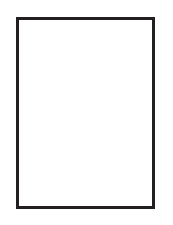
\includegraphics{photo.eps}}{\small\quad {\bf First Author [\textcolor{blue}{First-Name Surname}]}  \textcolor{blue}{Biographies should be limited to one paragraph consisting of sequentially ordered list of degrees, including the specialties and years achieved; sequentially ordered places of employ concluding with current employment; association with any refereed journals or conferences; major professional and/or academic achievements, i.e., best paper awards, etc.; current research interests. The resolution of the author' photo should be 600 dpi.}] }\\[1mm]}

\noindent\parbox{8.3cm}{\parpic{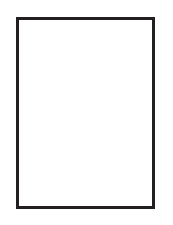
\includegraphics{photo.eps}}{\small\quad {\bf second Author [First-Name Surname]}  Content Content Content Content Content Content Content Content Content Content Content Content Content Content Content Content Content Content Content Content Content Content Content Content Content Content Content Content Content Content Content Content Content Content Content Content Content Content Content Content Content Content Content Content Content Content Content Content Content Content Content Content Content Content] }\\[1mm]}

\noindent\parbox{8.3cm}{\parpic{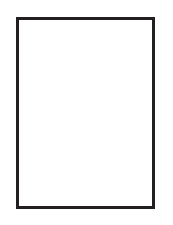
\includegraphics{photo.eps}}{\small\quad {\bf third Author [First-Name Surname]}  Content Content Content Content Content Content Content Content Content Content Content Content Content Content Content Content Content Content Content Content Content Content Content Content Content Content Content Content Content Content Content Content Content Content Content Content Content Content Content Content Content Content Content Content Content Content Content Content Content Content Content Content Content Content] }\\[1mm]}


%���䵽������������
%\textcolor{white}{text text text text text text text text text text text text text text  text text text text text text text text text text text text text text text text text text  text text text text text text text text text text text text }
\label{last-page}
\end{multicols}
\label{last-page}
\end{document}
